\documentstyle[art10,titlepage,makeidx,twoside,EPSF/epsf,mytabbing]{j-article}
\makeindex
\pagestyle{myheadings}
\oddsidemargin=0cm
\evensidemargin=0cm

% A4 size
\textwidth=16cm
\textheight=24cm
\topmargin=-1.5cm
\oddsidemargin= 0.7cm
\evensidemargin=0.7cm

% Letter size
%\topmargin=0.5cm
%\textwidth=17.6cm
%\textheight=23cm
%\oddsidemargin= 0.2cm
%\evensidemargin=0.2cm

\parindent=10mm
\parskip=1mm
%\baselineskip 14pt

\setcounter{totalnumber}{3}
\renewcommand{\topfraction}{0.99}       % 85% of a page (from page
                                        % top)
                                        % can be occupied by tbl / fig
                                        %
\renewcommand{\bottomfraction}{0.99}    % 85% of a page (from page
                                        % bottom)
                                        % can be occupied by tbl / fig
\renewcommand{\textfraction}{0.0}      % text shoud occupy 15% or
                                        % more in
                                        % a page
%\renewcommand{\floatpagefraction}{0.99} % 70% or more shoud occupy in
                                        % a
                                        % a float page


\jintercharskip=0pt plus3.0pt minus1pt%

\begin{document}

\newcommand{\ptext}[1]
{\tt \begin{quote} \begin{tabbing} #1 \end{tabbing} \end{quote} \rm}

\newcommand{\desclist}[1]{
\begin{list}{ }{\setlength{\rightmargin}{0mm}\topsep=0mm\partopsep=0mm}
\item #1
\end{list}
\vspace{3mm}}

\newcommand{\functiondescription}[4]{
\index{#1}
{\bf #1} \em #2 \rm \hfill [#3] 
\ifx#4\null \\ \else\desclist{#4}\fi
}

\newcommand{\longdescription}[3]{
\index{#1}
\begin{tabbing}
{\bf #1} 
\em #2
\rm
\end{tabbing}
\desclist{#3}
}

\newcommand{\funcdesc}[3]{\functiondescription{#1}{#2}{$@4X?t(J}{#3}}
\newcommand{\macrodesc}[3]{\functiondescription{#1}{#2}{$@%^%/%m(J}{#3}}
\newcommand{\specialdesc}[3]{\functiondescription{#1}{#2}{$@FC<l(J}{#3}}
\newcommand{\methoddesc}[3]{\functiondescription{#1}{#2}{$@%a%=%C%I(J}{#3}}
\newcommand{\vardesc}[2]{\functiondescription{#1}{}{$@JQ?t(J}{#2}}

\newcommand{\fundesc}[2]{\functiondescription{#1}{#2}{$@4X?t(J}{\hspace{0mm}}}
\newcommand{\macdesc}[2]{\functiondescription{#1}{#2}{$@%^%/%m(J}{\hspace{0mm}}}
\newcommand{\spedesc}[2]{\functiondescription{#1}{#2}{$@FC<l(J}{\hspace{0mm}}}
\newcommand{\metdesc}[2]{\functiondescription{#1}{#2}{$@%a%=%C%I(J}{\hspace{0mm}}}

\newcommand{\constdesc}[2]{\functiondescription{#1}{}{$@Dj?t(J}{#2}}

\newcommand{\classdesc}[4]{	%class, super slots description
%\vspace{5mm} 
\index{#1}
{\Large {\bf #1 }} \hfill [$@%/%i%9(J]  %super
\begin{tabbing}
\hspace{30mm} :super \hspace{5mm} \= {\bf #2} \\
\hspace{30mm} :slots \> #3 
\end{tabbing}
\vspace{4mm}
\desclist{#4}}

\newenvironment{refdesc}{
 \vspace{5mm} \parindent=0mm \topsep=0mm \parskip=0mm \leftmargin=10mm}{
             \parindent=10mm \topsep=3mm \parskip=1mm \leftmargin=0mm }


\title{\LARGE \bf EusLisp \\
{\large \bf version 7.27} \\
\bf $@%j%U%!%l%s%9%^%K%e%"%k(J \\
\vspace{5mm}
\normalsize
ETL-RM-87-06E \\
Feb,Jun/1989, Jun,Sep/1990, Oct/1991, Oct/1992  \\ }
\author{$@>>0f!!=S9@(J \\
{\small $@DL>&;:6H>J!!9)6H5;=Q1!(J}\\
$@EE;R5;=QAm9g8&5f=j(J \\
$@CNG=%7%9%F%`It!!<+N'%7%9%F%`8&5f<<(J}
\thispagestyle{empty}
\maketitle
\pagenumbering{roman}
\tableofcontents
% \listoffigures
% \listoftables
\bibliographystyle{plain}
\newpage
\pagenumbering{arabic}
\part{EusLisp $@4pK\(J}
\markboth{EusLisp $@%j%U%!%l%s%9%^%K%e%"%k(J (Part II)}{$@$O$8$a$K(J}
\newpage
%
%
\newpage
\section{Multithread\label{mthread}}
\markright{\arabic{section}. Multithread}

The multithread is the concurrent and asynchronous programming facility
on the Solaris operating system. 
Asynchronous programming is required for programs to respond to
external events via multiple sensors occurring independently of
the program's state.
Parallel programming is effective to improve performance of
computation bound processing such as image processing and interference
checking in path planning.

\subsection{Design of Multithread EusLisp}
\subsubsection{ Multithread in Solaris 2 operating system}
Multithread EusLisp (MT-Eus) runs on the Solaris 2 operating system
with one or more processors.  Solaris's threads are units for allocating
CPU in a traditional UNIX process, having shared memory and different
contexts. %{\cite Solaris-thread}.
The thread library provided by the Solaris OS allocates each
thread to a single LWP (light weight process), which is a kernel
resource.
The Unix kernel schedules the allocation of  LWPs to one or more
physical CPUs based on thread priorities assigned to each thread. 
Fig.\ref{threadmodel} depicts the relations between threads, LWPs, and CPUs.
Two major changes in the design of the contexts and the memory management
of EusLisp have been made to upgrade it to multithread capabilities.

\subsubsection{Context Separation}
MT-Eus allocates private stacks and contexts  to each threads
so that they can run independently of each other. Objects
such as symbols and conses are allocated in the shared heap
memory as in sequential EusLisp.
Therefore, thread-private data such as block labels,
catch tags, and local variables 
are protected from other threads, whereas  values (objects) 
pointed by global variables are visible to all threads allowing
information exchange among threads.

\begin{figure}[b]
\begin{center}
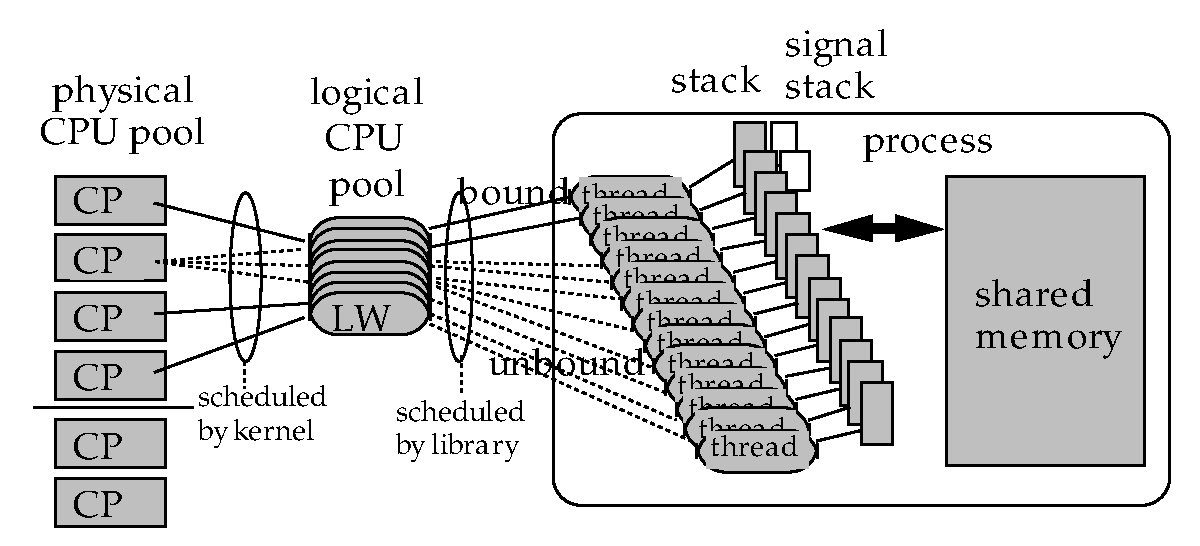
\includegraphics[width=13cm]{fig/threadfig.ps}
%\mbox{
%\epsfxsize=13cm
%\epsfbox{fig/threadfig.ps}
%}

\caption{Solaris operating system's thread model}\label{threadmodel}
\end{center}
\end{figure}

A context consists of a C-stack, a binding-stack and frame 
pointers that chain lexical blocks such as {\tt lambda, block, catch,
let, flet}, and so on,  and is established when a new thread
is created. Since more than one context can be active at
the same time on a real multi-processor machine, we cannot
hold a single pointer to the current context in a global variable.
Rather we have to add one more argument to every internal
function to transfer the context pointer  from the topmost eval
to the memory manager at the bottom.

\subsubsection{Memory Management}
EusLisp adopts a Fibonacci buddy memory management scheme in a
single heap for every type of object. 
After running programs having
different memory request characteristics, we have been convinced that
Fibonacci buddy can allocate objects of various sizes equally fast,
garbage-collects quickly without copying , and exhibits high memory
utilization (the internal loss is 10 to 15\% and the
external loss is negligible).
For multithreading, the second point, i.e., non-copying GC, is very
important.
If addresses of objects were changed by copying-GC, pointers in the
stack and CPU registers of all thread contexts would have to be
redirected to new locations, which is impossible or very difficult. 

All memory allocation requests are handled by the {\tt alloc} function at the
lowest level.
{\tt Alloc} does mutex-locking because it manipulates the global
database of free lists.
Since we cannot predict when a garbage
collection begins and which thread causes it, every thread must prepare
for sporadic GCs.  All pointers to living objects have to be arranged
to be accessible by the GC anytime to prevent them from being reclaimed
as garbage.  This is done by storing the pointers to the most recently
allocated objects in fixed slots of each context, instead of trusting
they are maintained on the stacks.

Fig. \ref{parathreads} illustrates flow of threads requesting memory and forked inside
GC to process marking and sweeping in parallel.
Note that threads that do not request memory or manipulate pointers
can run in parallel with the GC,
improving real-time response of the low-level tasks such as signal
processing and image acquisition.

\begin{figure}
\begin{center}
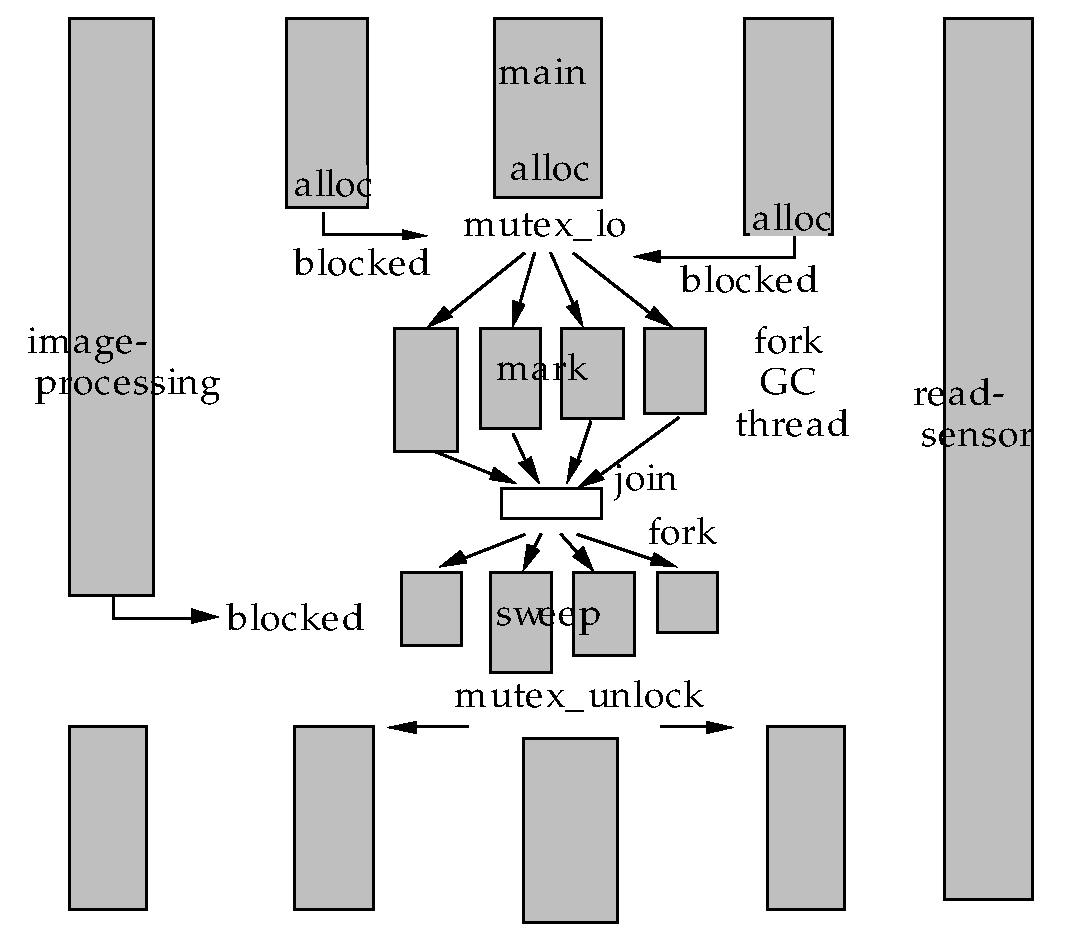
\includegraphics[width=120mm]{fig/parathreads.ps}
%\epsfile{file=fig/parathreads.ps,width=120mm}
\caption{Parallel threads requesting memory and GC running in parallel}\label{parathreads}
\end{center}
\end{figure}

\subsection{Asynchronous and Parallel Programming Constructs}
\subsubsection{Thread Creation and Thread Pool}
In order for Solaris to execute a program in parallel on many
processors, the program needs to be written as a collection
of functions, each of which is executed by a thread dynamically
created in a process.  Although the time required for thread
creation is faster than process creation, it takes a few
mili-seconds for EusLisp to start off a thread after allocating
stacks and setting a page attribute for detecting stack-overflow.
Since this delay, which should be compared to a function invocation,
is intolerable, sufficient number of threads are created by
the {\tt make-thread} function beforehand and put in 
the system's thread pool,
eliminating the need for system calls at evaluation time.
Each thread in the thread pool is represented by a thread object,
as depicted in Fig.\ref{threadobj},
consisted of thread-id, several semaphores for synchronization,
and slots for argument and evaluation result transfer.

\begin{figure}
\begin{center}
\begin{tabular}{c c}
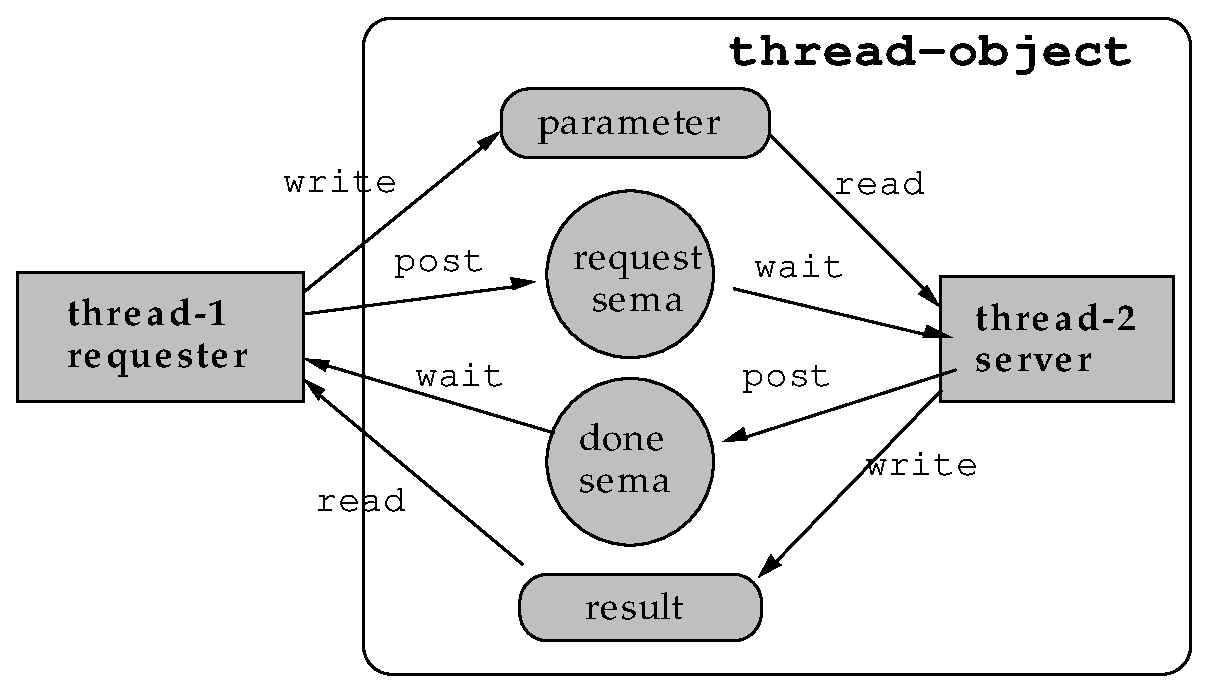
\includegraphics[width=7.5cm]{fig/threadobj.ps} &
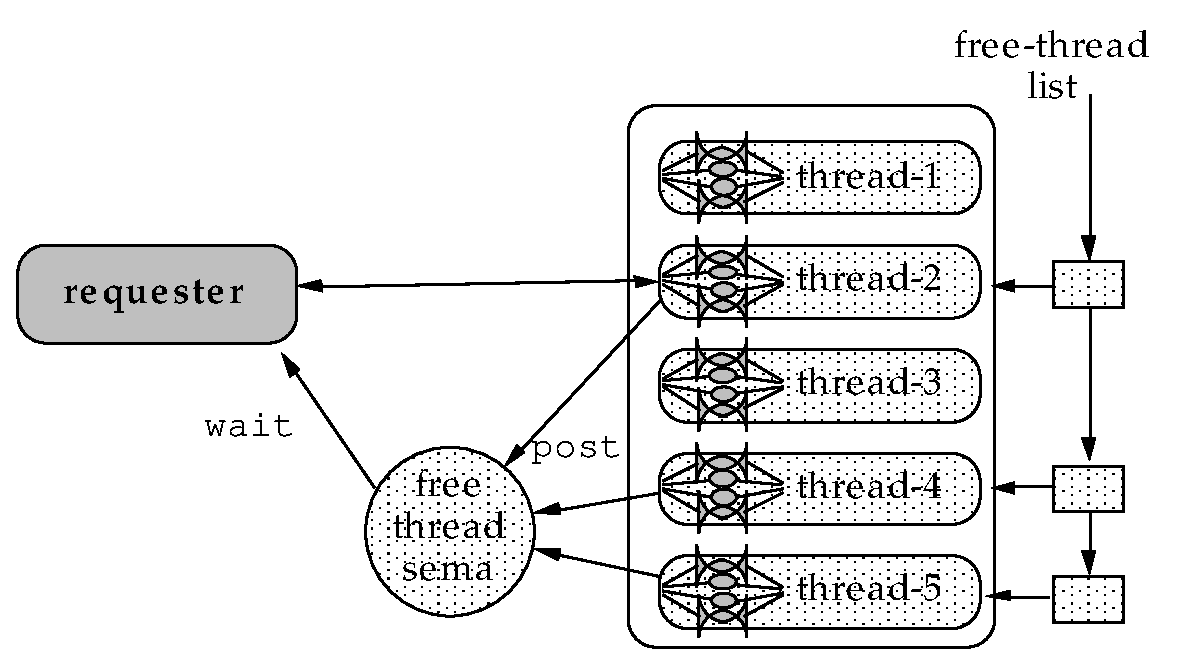
\includegraphics[width=7.5cm]{fig/threadpool.ps} \\
%\epsfile{file=fig/threadobj.ps,width=7.5cm} &
%\epsfile{file=fig/threadpool.ps,width=7.5cm} \\
\end{tabular}
\end{center}
\caption{\label{threadobj}Thread-object for transferring control and data between threads (left) and the collection of threads put in the thread-pool.}
\end{figure}

\subsubsection{Parallel Execution of Threads}
For the allocation of parallel computation to threads, the thread function
is used.
Thread takes one free thread out of the thread pool,
transfers arguments via shared memory, wakes up the thread by signaling
the semaphore as indicated in fig. \ref{threadobj},
and returns a thread object to the caller without blocking.
The woken-up thread begins evaluation of
the argument running in parallel to the calling thread.
The caller uses
{\tt wait-thread} to receive the evaluation result from the forked thread.
The {\tt plist} macro is a more convenient form to describe parallel 
evaluation of arguments.
{\tt Plist} attaches threads to evaluate each argument
and lists up results after waiting for all threads to finish evaluation.

\subsubsection{Synchronization primitives}
MT-Eus has three kinds of synchronization primitives,
namely {\em mutex locks, condition variables}, and {\em semaphores}.
Mutex locks  are used to serialize accesses to shared variables
between threads.
Condition variables allow a thread to wait for a condition to become
true in a mutex-locked section by temporarily releasing and re-acquiring 
the lock.
Semaphores are used to inform occurrences of events, or to control
sharing of finite resources.
These synchronization primitives cause voluntary context switching,
while the Solaris kernel generates involuntary task switching
on a time-sliced scheduling basis.

\begin{figure}
\begin{center}
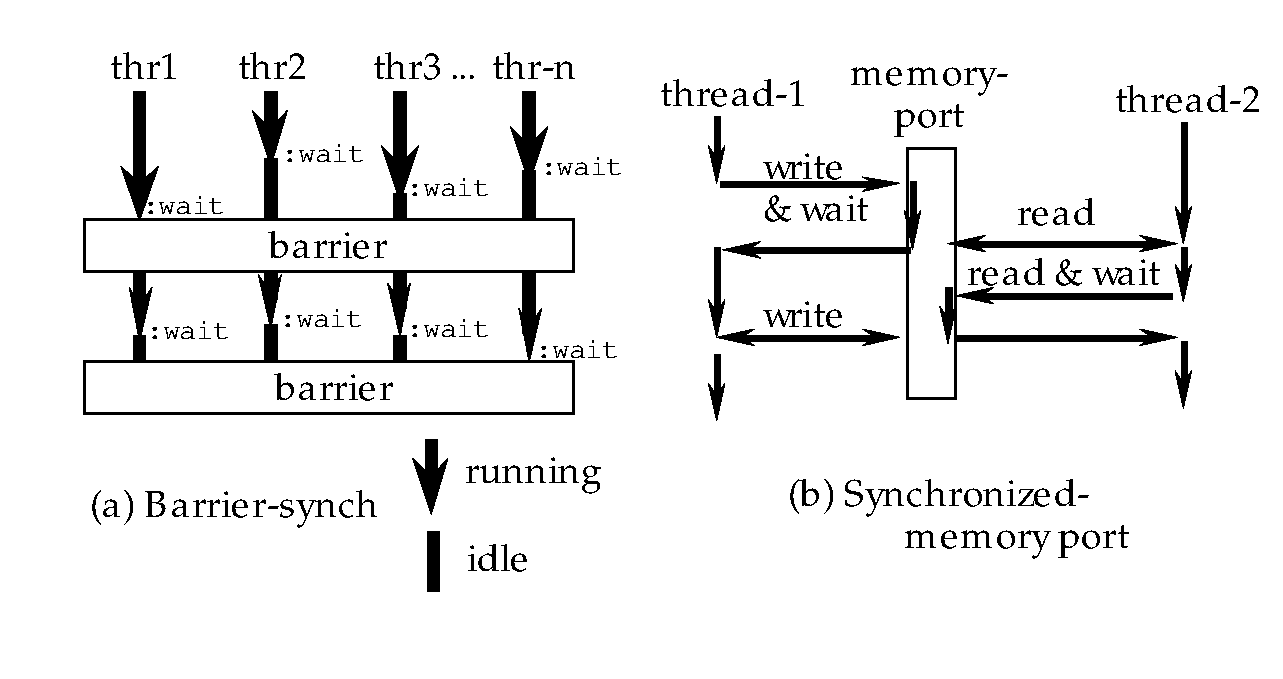
\includegraphics[width=130mm]{fig/synchports.ps}
%\epsfile{file=fig/synchports.ps,width=130mm}
\caption{Barrier synchronization and synchronozed memory port}
\label{synchports}
\end{center}
\end{figure}

\subsubsection{Barrier synchronization}
{\em Barrier-synch} is a mechanism for more than two threads to synchronize
at the same time (Fig. \ref{synchports}).
For this purpose, an instance of the barrier class
is created and threads that participate in
the synchronization register themselves in the object.
Then, each thread sends the {\tt :wait} message to the barrier object,
and the thread is blocked.
When the last thread registered in the object sends its
{\tt :wait} message, the waits are released and all waiting
threads get a return value of T.
Barrier-sync plays an important role of global clocking in a
multi-robot simulation.

\subsubsection{Synchronized memory port}
Synchronized memory port is a kind of stream to exchange data
between threads (Fig. \ref{synchports}).
Since all threads in a process share the
heap memory, if one thread binds an object to a global variable,
it  instantly becomes visible to other threads.
However, shared memory lacks capability to send events that the
global data is updated. Synchronized memory port ensures this 
synchronization for accessing a shared object. A synchronized
memory port object consists of one buffer slot and two semaphores
used for synchronizing  read and write.

\subsubsection{Timers}
Real-time programs often require functions to execute at
predetermined timing or to repeat in particular intervals.
Sequential EusLisp could run user' functions triggered by
signals generated periodically by Unix's interval timers.
This preemption can cause deadlock in MT-Eus,
because interruption may occur within a mutex-ed block.
Therefore, control must be transferred at secured points
such as at the beginning of {\tt eval}.
To avoid delays caused by the above synchronization,
MT-Eus also provides signal-notification via semaphores.
In other words, the signal function takes either a function or
a semaphore that is called or posted upon the signal arrival.
Since the semaphore is posted at the lowest level, latency
for synchronization is minimal.

The following a example image processing program
coded by using the multithread facilities.
Image input thread and filtering
threads are created. samp-image takes image data periodically
by waiting for samp-sem to be posted every 33msec.
Two threads synchronize via read-and-write of a thread-port.
Filter-image employs two more threads for parallel computation
of filtering.

\begin{quote}
\begin{verbatim}
(make-threads 8)
(defun samp-image (p)
   (let ((samp-sem (make-semaphore)))
        (periodic-sema-post 0.03 samp-sem)
        (loop (sema-wait samp-sem)
              (send p :write (read-image))))
(defun filter-image (p)
  (let (img)
       (loop (setf img (send p :read))
             (plist (filter-up-half img)
                    (filter-low-half img)))))
(setf port (make-thread-port))
(setf sampler (thread #'samp-image port))
(setf filter (thread #'filter-image port))
\end{verbatim}
\end{quote}

\subsection{Measured Parallel Gains}

Table. \ref{paragain} shows the parallel execution performance
measured on a Cray Supserserver configured with 32 CPUs.
Linear parallel gain was obtained for the compiled Fibonacci function,
because there is no shared memory access and  the program code
is small enough to be fully loaded onto the cache memory of
each processor.
Contrally, when the same program was interpreted, linearly
high performance could not be attained, since memory access
scatters. Further, some programs that frequently refer to 
shared memory and request memory allocation cannot exhibit better
performance than a single processor execution.
This can be understood as the result of frequent  cache memory
purging.

\begin{table}
\begin{center}
\begin{tabular}{|l|r|r|r|r|c|}  \hline
processors & 1 & 2 & 4 & 8 & GC (ratio) \\ \hline
(a) compiled Fibonacci & 1.0 & 2.0 & 4.0 & 7.8 & 0 \\ \hline
(b) interpreted Fibonacci & 1.0 & 1.7 & 2.7 & 4.4 & 0 \\ \hline
(c) copy-seq & 1.0 & 1.3 & 0.76 & 0.71 & 0.15 \\ \hline
(d) make-cube & 1.0 & 0.91 & 0.40 & 0.39 &  0.15 \\ \hline
(e) interference-check & 1.0 & 0.88 & 0.55 & 0.34 & 0.21 \\ \hline
\end{tabular} \\
\caption{\label{paragain}Parallel gains of programs executed on multi-processors}
\end{center}
\end{table}

\subsection{Thread creation}
A thread is a unit for assigning computation, usually evaluation
of a lisp form.
Threads in EusLisp are represented by instances of
the {\bf thread} class.
This object is actually a control port of a thread 
to pass arguments and result, and let it start evaluation,
rather than the thread's entity representing the context.

\begin{refdesc}

\funcdesc{sys:make-thread}{num \&optional (lsize 32*1024) (csize lsize)}{
creates {\em num} threads with {\em lsize} words of Lisp stack
and {\em csize} words of C stack, and put them in the system's
thread pool.
All the threads in the thread pool is bound to sys:*threads*,
which is extended each time {\bf make-thread} is called.
By the {\bf thread} function, a computation is assigned to one
of free threads in the thread pool.
Therefore it is not a good idea to change stack sizes
from thread to thread,
since you cannot control which thread is assigned to a specific
computation.}

\vardesc{sys:*threads*}{
returns the list of all the threads created by {\bf make-threads}.}

\funcdesc{sys::free-threads}{}{
returns the list of threads in the
free thread pool.
If the result is NIL, new commitment of a task to a thread
is blocked until any currently running threads finish evaluation
or new threads are created by {\bf make-thread} in the free thread pool.}

\funcdesc{sys:thread}{func \&rest args}{
picks up one free thread from the thread pool, and assigns it
for evaluation of {\em (func . args)}.
{\bf Sys:thread} can be regarded as asynchronous {\bf funcall},
since {\bf sys:thread} applies {\em func} to the spread list
of {\em args} but it does not accept the result of the
function application.
Rather, {\bf sys:thread} returns the thread object assigned to
the funcall, so that the real result can be obtained later
by {\bf sys:wait-thread}.}
\begin{quote}
\begin{verbatim}
(defun compute-pi (digits) ...)
(setq trd (sys:thread \#'compute-pi 1000)) ;assign compute-pi to a thread
...  ;; other computation 
(sys:wait-thread trd) ;get the result of (compute-pi 1000)
\end{verbatim}
\end{quote}

\funcdesc{sys:thread-no-wait}{func \&rest args}{
assigns computation to one of free threads.
The thread is reclaimed in the free thread pool when
it finishes evaluation without being {\bf wait-thread}'ed.}

\funcdesc{sys:wait-thread}{thread}{
waits for {\em thread} to finish evaluation of funcall given
by the {\bf sys:thread} function, and retrieves the result
and returns it.
{\bf Sys:wait-thread} is mandatory if the thread is assigned
evaluation by {\bf sys:thread} because the thread is not returned
to the free thread pool until it finishes transferring the result.}
 
\macrodesc{sys:plist}{\&rest forms}{evaluates {\em forms} by different
threads in parallel and waits for the completion of all evaluation,
and the list of results is returned.
{\bf Sys:plist} may be regarded as {\em parallel-list} except that
each form listed must be a function call.}


\end{refdesc}

\subsection{Synchronization}

Among Solaris operating systems four synchronization primitives for
multithread programs, EusLisp provides mutex locks, conditional variables,
and semaphores. Reader-writer lock is not available now.

Based on these primitives, higher level synchronization mechanisms,
such as synchronized memory port and barrier synchronization, are realized.

\begin{refdesc}
\funcdesc{sys:make-mutex-lock}{}{
makes a mutex-lock and returns it. A mutex-lock is represented by an
integer-vector of six elements.}
\funcdesc{sys:mutex-lock}{mlock}{
locks the mutex lock {\em mlock}.
If the {\em mlock} is already locked by another thread,
{\em mutex-lock} waits for the lock to be released.}

\funcdesc{sys:mutex-unlock}{mlock}{
releases {\em mlock} and let one of other threads waiting for this
lock resume running.}

\macrodesc{sys:mutex}{mlock \&rest forms}{
Mutex-lock and mutex-unlock have to be used as a pair.
{\bf Mutex} is a macro that brackets a critical section.
{\em Mlock} is locked
before evaluating {\em forms} are evaluated,
and the lock is released when the evaluation finishes.
This macro expands to the following progn form.
Note that {\bf unwind-protect} is used to ensure unlocking
even an error occurs during the evaluation of {\em forms}.
}
\begin{quote}
\begin{verbatim}
  (progn
      (sys:mutex-lock mlock)
      (unwind-protect
          (progn . forms)
          (sys:mutex-unlock mlock)))
\end{verbatim}
\end{quote}

\funcdesc{sys:make-cond}{}{makes a condition variable object
which is an integer vector of four elements.
The returned condition variable is in unlocked state.}

\funcdesc{sys:cond-wait}{condvar mlock}{
waits for {\em condvar} to be signaled.
If {\em condvar} has already been acquired by another thread,
it releases {\em mlock} and waits for {\em condvar} to be signaled.}
\funcdesc{sys:cond-signal}{condvar}{signals the {\em condvar} condition variable.}
\funcdesc{sys:make-semaphore}{}{makes a semaphore object
which is represented by an integer vector of twelve elements.}
\funcdesc{sys:sema-post}{sem}{ signals {\em sem}.}
\funcdesc{sys:sema-wait}{sem}{waits for the {\em sem} semaphore to be posted.}

\classdesc{sys:barrier-synch}{propertied-object}{
threads n-threads count barrier-cond threads-lock count-lock}
{represents a structure for barrier-synchronization. Threads waiting
for the synchronization are put in {\em threads} which is mutually excluded
by {\em threads-lock}.
When a {\bf barrier-synch} object is created,
{\em count} is initialized to zero.
Synchronizing threads are put in the {\em threads} list by sending {\tt :add}
message.
Sending {\tt :wait} to this barrier-sync object causes {\em count} to be
incremented, and the sending thread is put in the wait state.
When all the threads in {\em threads} send the {\tt :wait} message,
the waits are unblocked and all threads resume execution.
The synchronization is implemented by the combination of
the {\em count-lock} mutex-lock and the {\em barrier-cond}
condition-variable.}

\methoddesc{:init}{}{initializes this barrier-synch object. Two mutex-lock
and one condition-variable are created.}
\methoddesc{:add}{thr}{adds the {\em thr} thread in the {\em threads} list.}
\methoddesc{:remove}{thr}{removes the {\em thr} thread of the {\em threads} list.}
\methoddesc{:wait}{}{waits for all threads in the {\em threads} list
to issue {\tt :wait}.}

\classdesc{sys:synch-memory-port}{propertied-object}{
sema-in sema-out buf empty lock}{
realizes the one-directional synchronized memory port,
which synchronizes for two threads
to transfer datum via this object.
Control transfer is implemented by using semaphores.}

\methoddesc{:read}{}{reads datum buffered in this synch-memory-port.
If it has not been written yet, the :read blocks.}
\methoddesc{:write}{datum}{writes {\em datum} in the buffer.
Since only one word of buffer is available,
if another datum has already been written and not yet read out,
:write waits for the datum to be transferred by :read.}
\methoddesc{:init}{}{initializes this synch-memory-port
where two semaphores  are created and :write is made acceptable.}

\end{refdesc}

\section{Xwindow Interface}
\markright{\arabic{section}. Xwindow}
The Xwindow interface on EusLisp becomes available when EusLisp is
invoked by the name of {\tt 'eusx'}.
\footnote{Eusx is a symbolic link to eus.}
The "DISPLAY" environment variable should be properly set to your Xserver,
since eusx tries to connect to Xserver referencing
the "DISPLAY" environment variable when it starts up.

EusLisp defines three levels of xwindow interface:
(1) Xlib functions, (2) Xlib classes, and (3) XToolKit classes.
All the xwindow functions described in this section and the following
XToolKit section are contained in the "X" package.
The function names of the original Xlib are changed so that
all constituent letters are converted to upcase
and the first 'X' prefix is removed.
For example, {\tt XdefaultGC} is named {\tt X:DEFAULTGC},
not {\tt X:XDEFAULTGC}.

The Xlib functions are defined as foreign functions
as the lowest level interface to Xwindow system.
These Xlib functions should be used carefully, 
since parameter type check or parameter number check is not performed.
For an instance, all the Xlib call requests {\tt x:*display*} argument
to identify the connection to Xserver, and if you forget it, Xlib reports
an error and the process dies.
The second level interface, Xlib classes are provided
to avoid this inconvenience and to make the interface object-oriented.
%By instantiating the xwindow class, you will get a window on a screen,
%and sending messages to the instance, you can draw lines, strings, or whatever
%in it.
This section focuses on this second level interface.
Even higher level xwindow library called XToolKit is explained 
in the next section.

Classes described in this section have the following inheritance
hierarchy.

\begin{quote}
\begin{verbatim}
propertied-object
   viewsurface
      x:xobject
         x:gcontext
         x:xdrawable
             x:xpixmap
             x:xwindow
   colormap
\end{verbatim}
\end{quote}

\subsection{\label{xvariables}Xlib global variables and misc functions}
\begin{refdesc}
\vardesc{x:*display*}{X's display ID (integer).}
\vardesc{x:*root*}{default root window object. }
\vardesc{x:*screen*}{default screen ID (integer).}
\vardesc{x:*visual*}{default visual ID (integer).}
\vardesc{x:*blackpixel*}{black pixel = 1}
\vardesc{x:*whitepixel*}{white pixel = 0}
\vardesc{x:*fg-pixel*}{default foreground pixel referenced at window creation,
normally {\tt *blackpixel*}.}
\vardesc{x:*bg-pixel*}{background pixel referenced at window creation,
normally {\tt *whitepixel*}}
\vardesc{x:*color-map*}{the system's default color-map}
\vardesc{x:*defaultGC*}{the default gcontext referenced at pixmap creation.}
\vardesc{x:*whitegc*}{GC whose foreground color is white.}
\vardesc{x:*blackgc*}{GC whose foreground color is black.}

% \vardesc{*gray-gc*}{half-tone GC}
\vardesc{*gray-pixmap*}{the result of {\tt (make-gray-pixmap 0.5)}}
\vardesc{*gray25-pixmap*}{16x16 pixmap,
a quarter of pixels are {\tt *fg-pixel*} and three quarters {\tt *bg-pixel*}.}
\vardesc{*gray50-pixmap*}{16x16 pixmap, a half of pixels are {\tt *fg-pixel*}.}
\vardesc{*gray75-pixmap*}{16x16 pixmap, three quarters of pixels are black.}
\vardesc{*gray25-gc*}{25\% gray GC made from  {\tt *gray25-pixmap*}.}
\vardesc{*gray50-gc*}{50\% gray GC made from  {\tt *gray50-pixmap*}.}
\vardesc{*gray75-gc*}{75\% gray GC made from  {\tt *gray75-pixmap*}.}
\vardesc{*gray*}{{\tt "\#b0b0b0"}}
\vardesc{*bisque1*}{{\tt "\#ffe4c4"}}
\vardesc{*bisque2*}{{\tt "\#eed5b7"}}
\vardesc{*bisque3*}{{\tt "\#cdb79e"}}
\vardesc{*lightblue2*}{{\tt "\#b2dfee"}}
\vardesc{*lightpink1*}{{\tt "\#ffaeb9"}}
\vardesc{*maroon*}{{\tt "\#b03060"}}
\vardesc{*max-intensity*}{65535}
\vardesc{font-cour8}{{\tt (font-id "*-courier-medium-r-*-8-*")}}
\vardesc{font-cour10}{{\tt (font-id "*-courier-medium-r-*-10-*")}}
\vardesc{font-cour12}{{\tt (font-id "*-courier-medium-r-*-12-*")}}
\vardesc{font-cour14}{{\tt (font-id "*-courier-medium-r-*-14-*")}}
\vardesc{font-cour18}{{\tt (font-id "*-courier-medium-r-*-18-*")}}
\vardesc{font-courb12}{{\tt (font-id "*-courier-bold-r-*-12-*")}}
\vardesc{font-courb14}{{\tt (font-id "*-courier-bold-r-*-14-*")}}
\vardesc{font-courb18}{{\tt (font-id "*-courier-bold-r-*-18-*")}}
\vardesc{font-helvetica-12}{{\tt (font-id "*-Helvetica-Medium-R-Normal-*-12-*")}}
\vardesc{font-lucidasans-bold-12}{{\tt (font-id "lucidasans-bold-12")}}
\vardesc{font-lucidasans-bold-14}{{\tt (font-id "lucidasans-bold-14")}}
\vardesc{font-helvetica-bold-12}{{\tt (font-id "*-Helvetica-Bold-R-Normal-*-12-*")}}
\vardesc{font-a14}{{\tt (font-id "*-fixed-medium-r-normal-*-14-*")}}

%\vardesc{x:*reversevideo*}{}
\vardesc{x:*xwindows*}{a list of all windows including subwindows
created and maintained by EusLisp.}
\vardesc{x:*xwindow-hash-tab*}{a hash table to look up the xwindow object
by its drawable ID.
In the event structure obtained by {\tt x:nextevent} is a window ID,
and {\tt x:window-main-loop} calls {\tt x:event-window} to know
the corresponding xwindow object using this table.}
%\vardesc{x:gcval}{}

\funcdesc{xflush}{}{
sends all commands retained in the Xlib command buffer to Xserver.
Since Xlib buffers output to Xserver,
commands you issued commands to Xserver are not executed immediately.
This is necessary to decrease network traffic and the frequency
of process switching.
To flush the command buffer to see the effects of the commands,
use {\bf xflush} or send {\bf :flush}
message to  xwindow objects.
}
\funcdesc{find-xwindow}{subname}{
Each xwindow may have name specified at the creation time.
Find-xwindow looks in the *xwindows* list and returns a list
of windows that have 'subname' as a substring
of its name. }

\end{refdesc}

\subsection{Xwindow}

\begin{refdesc}

\classdesc{Xobject}{geometry:viewsurface}{}{
The common super class for all the Xwindow related classes.
Currently, no slots variables and methods are defined.}

\classdesc{Xdrawable}{Xobject}
{(drawable  \hspace{10mm} \=  ; drawable  ID \\
 \> gcon \>  ; this drawable's default graphic context object\\
\> bg-color \> ; background color \\
\> width height \> ; horizontal and vertical dimensions in dots}
{{\bf Xdrawable} defines rectangular regions where graphics objects such as
lines and strings can be drawn.
{\bf Xdrawable} is an abstract class to define
common methods for xwindow and xpixmap,
and instantiation of this class has no effect.}

\methoddesc{:init}{id}{
{\em Id} is set to the {\em drawable} slot as the ID of this drawable.
A new GC (graphic context) is created and set to {\em gcon} as 
the default GC of this drawable object.}
\methoddesc{:drawable}{}{returns drawable id.}
\methoddesc{:flush}{}{flushes commands retained in the Xlib's buffer.}
\methoddesc{:geometry}{}{
returns the list of seven geometric attributes,
{\em root-window-id, x-position, y-position,
width, height, border-width} and {\em visual's depth}.}
\methoddesc{:height}{}{
returns the height (dots in y direction) of this drawable.}
\methoddesc{:width}{}{
returns width (dots in x direction) of this drawable.}
\methoddesc{:gc}{\&rest newgc}{
If no {\em newgc} is given, the current gc object is returned.
If {\em newgc} is an instance of gcontext,
it is set to the gc of this drawable.
Otherwise, {\em newgc} is regarded as a message and  sent to
the current gc.}
\methoddesc{:pos}{}{returns an integer vector representing 
the position of this drawable.
The position is always defined relative to the 
parent window, and windows created as direct subwindows of the root
window under the intervention of the window manager return the constant
coordinates in their surrounding title window regardless to their
true position in the root.}
\methoddesc{:x}{}{returns the {\em x} coordinate of this drawable relatively to
the parent window.}
\methoddesc{:y}{}{returns the {\em y} coordinate of this drawable relatively to
the parent window.}

\methoddesc{:copy-from}{drw}{
{\em Drw} is another drawable object (xwindow or pixmap).
The contents of {\em drw} is copied to this drawable.}

\begin{figure}
\begin{center}
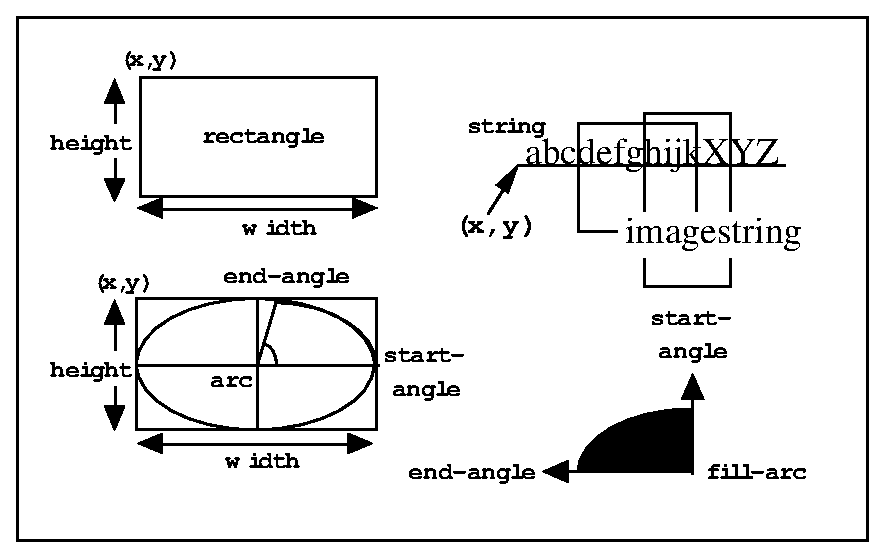
\includegraphics[height=6cm]{fig/xdraw.ps}
%\epsfile{file=fig/xdraw.ps,height=6cm}
%\mbox{
%\epsfysize=6cm
%\epsfbox{fig/xdraw.ps}
%}
\end{center}
\caption{drawing primitives\label{xdraw}}
\end{figure}


\methoddesc{:point}{x y \&optional (gc gccon)}{
draws a point at $(x, y)$ with optional {\em gc}.}
\methoddesc{:line}{x1 y1 x2 y2 \&optional (gc gcon)}{
draw a line from {\em (x1, y1)} to {\em (x2, y2)}
with optional {\em gc}. {\em x1, y1, x2,} and{\em y2} must be integers.}
\methoddesc{:rectangle}{x y width height \&optional (gc gcon)}{
draws a rectangle whose center is located at {\em (x, y)}
and size is specified by {\em width} and {\em height}.}
\methoddesc{:arc}{x y width height angle1 angle2 \&optional (gc gcon)}{
draws an elliptic arc whose center is {\em (x, y)} and starting angle at 
{\em angle1} and ending angle at {\em angle2}.
Angles should be given by radian.}
\methoddesc{:fill-rectangle}{x y width height \&optional (gc gcon)}{
fills in a rectangular region.}

\methoddesc{:fill-arc}{x y width height angle1 angle2 \&optional (gc gcon)}{
fills in an arc.
}
\methoddesc{:string}{x y str \&optional (gc gcon)}{
displays the string {\em str} starting at {\em (x, y)}. The background is
not filled.}
\methoddesc{:image-string}{x y str \&optional (gc gcon)}{
displays an imagestring of {\em str}. Imagestring fills background.}
\methoddesc{:getimage}{\&key x y width height (mask \#ffffffff) (format 2)}{
gets ximage from the server and returns the pixel data in a string.
The pixel data sent from the server is once stored in Xlib's ximage structure,
then copied to the string row by row.
The ximage structure is automatically destroyed.
The image string obtained by {\tt :getimage} can be used to make
a {\tt pixel-image}, which can be written to a file in the pbm formats
as described in section \ref{PBMfile}.}
\methoddesc{:putimage}{image \&key src-x src-y dst-x dst-y width height ((:gc g) gc)}{
puts {\em image} to the specified location in this drawable.
{\em image} is a string or a address pointing to an ximage structure.}
\methoddesc{:draw-line}{from to}{
is same as {\bf :line} method,
and provided for the compatibility with other viewsurface classes.}
\methoddesc{:line-width}{\&optional dots}{sets line-width of this drawable's
default GC. Use of the {\tt :gc :line-width} message is recommended.}
\methoddesc{:line-style}{\&optional dash}{sets line-style of this drawable's
default GC. Use of the {\tt :gc :line-style} is preferable.}
\methoddesc{:color}{\&optional c}{sets color of this drawable.}
%\methoddesc{:set-show-mode}{}{
%sets copy mode. this function usually uses for monochrome display.}
%\methoddesc{:set-erase-mode}{}{
%sets erase mode. this function usually uses for monochrome display.}
%\methoddesc{:set-xor-mode}{}{
%sets xor mode. this function usually uses for monochrome display.}
\methoddesc{:clear}{}{
clears full screen. this method calls {\tt :clear-area}}
\methoddesc{:clear-area}{\&key :x  :y :width :height :gc}{
clears a rectangle using the {\tt :fill-rectangle} method.}

\classdesc{Xpixmap}{Xdrawable}{}{Pixmap is a drawable that is often used
as a picture buffer or a background pattern.
Unlike xwindow, pixmap itself is not visible until it is copied to xwindow
or pixmap does not generate any event.}

\methoddesc{:init}{id}{initializes this pixmap.}
\methoddesc{:create}{\&key (width 500) (height 500) (depth 1) (gc *defaultgc*)}{
creates a {\em width} x {\em height} pixmap with {\em gc} as its
default GC.}
\methoddesc{:create-from-bitmap-file}{fname}{
creates a pixmap from a bitmap file.}
\methoddesc{:write-to-bitmap-file}{fname}{
writes the contents of this pixmap into a bitmap file,
which can be read back to create a pixmap by {\bf :create-from-bitmap-file}
method.}
\methoddesc{:destroy}{}{
destroys this pixmap and frees X resources.}

%%%%%% X W I N D O W
\classdesc{Xwindow}{Xdrawable}{(parent subwindows backing-pixmap event-forward)
}{{\bf Xwindow} defines visible rectangular regions of the screen.
It is inherited not only by {\bfx text-window} and {\bf canvas} where
any graphics objects can be drawn, but also by many {\bf panel-items}
and {\bf scroll-bars}, which look like graphics objects rather than windows.}

\longdescription{:create}{\&key ( \= (:parent *root*) \` [method] \\
\> (x 0) (y 0) (size 256) (width size) (height size) (border-width 2) \\
\> (save-under nil) (backing-store :always) (backing-pixmap nil)\\
\> (border *fg-pixel*) (background *bg-pixel*) \\
\> (map T) (gravity :northwest) \\
\> (title "WINDOW") (name title) \\
\> (font) \\
\> event-mask (:key :button :enterLeave :configure :motion)}
{creates and initializes a xwindow.
When {\em parent} is given, this window is created as a subwindow
of {\em parent}, and is registered in the {\em subwindows} list of
the {\em parent}.
{\em X, y, size, width, height} and {\em border-width} determine
the location and the dimensions of this window.
{\em Save-under} and {\em backing-store} control the Xserver's behaviors
taken upon when the window is re-mapped. {\em Save-under} is either
T or NIL, while {\em backing-store} is either {\tt :notUseful, :WhenMapped},
or {\em :Always}.
When {\em backing-pixmap} is T, a pixmap of the same size as this window
is created by EusLisp, and maintained as a backing-store in case
the Xserver does not have the capability of backing-store.
{\em Border} and {\em background} specify the {\em border\_pixel}
and {\em background\_pixel} attributes, respectively.
{\em Map} should be set NIL, if this window should not appear
immediately after its creation, as is the case many small windows 
are created as panel-buttons in a {\bf panel}.
{\em Title} is the window title which appears in the title bar of 
the window.
{\em Name} is the name of the window stored in the property-list
of this xwindow object and printed by the printer.
X's events reported to this window are determined by 
{\em Event-mask}, that is, either an integer representing a bit-coded event-mask
or a list of the following symbols:
{\tt :key, :button, :enterLeave, :motion} and {\tt :configure}.
If more precise control is needed, the following symbols for each event
can be specified: {\em :keyPress, :keyRelease, :ButtonPress, :ButtonRelease,
:EnterWindow, :LeaveWindow, :PointerMotion, :PointerMotionHint, 
:ButtonMotion, :KeyMapState, :Exposure, :VisibilityChange, :StructureNotify,
:ResezeRedirect, :SubstructureNotify, :SubstructureRedirect,
:FocusChange, :PropertyChange, :ColormapChange} and {\tt :OwnerGrabButton}.
{\tt :Key} enables both {\tt :keyPress} and {\tt :KeyRelease}, and
{\tt :button} enables both {\tt :ButtonPress} and {\tt :ButtonRelease}.
When an event is sent from the server, {\bfx window-main-loop} analyzes
the event structure and send the {\tt :KeyPress, :KeyRelease, :buttonPress,
:ButtonRelease, :EnterNotify, :LeaveNotify, :MotionNotify, :ConfigureNotify}
message to the window where the event occurred.}

\methoddesc{:map}{}{makes this xwindow and all the subwindows visible.}
\methoddesc{:unmap}{}{makes this xwindow and all the subwindows invisible.}
\methoddesc{:selectinput}{event-mask}{
{\em Event-mask} is either an integer or a list of eventmask symbols.
Each event corresponding to the bit turned-on or 
enumerated in the {\em event-mask} list
becomes to be reported to this window.}
\methoddesc{:destroy}{}{destroys this xwindow and frees X resource.
The corresponding entries in {\tt *xwindows*} and {\tt *xwindow-hash-tab*}
are also deleted so that this window object could be garbage-collected.
All subwindows are also deleted by sending {\tt :destroy}.
This window is dissociated from the subwindow list of the parent window.
The {\em drawable} ID is set to NIL.}
\methoddesc{:parent}{}{returns the parent window object.}
\methoddesc{:subwindows}{}{
returns the list of all the subwindows.
The subwindow most recently created comes first in the list.
Only the direct subwindows of this window are listed and
subwindows of the subwindows are not.}
\methoddesc{:associate}{child}{register the {\em child} window
as a subwindow of this window.}
\methoddesc{:dissociate}{child}{removes the {\em child} window
of the {\em subwindows} list.}

%\methoddesc{:save}{}{
%copies the content of this window to the backing-store pixmap.}
%\methoddesc{:refresh}{}{
%copies from the backing-store.}

\methoddesc{:title}{title}{
changes the title of this window.
Though the title is in the Xserver, it is maintained and displayed by
the window manager.}

\methoddesc{:attributes}{}{returns an integer-vector representing
the attributes of this window.}
\methoddesc{:visual}{}{returns the visual resource id for this window.} 
\methoddesc{:screen}{}{returns the screen resource id for this window.} 
\methoddesc{:root}{}{returns the root window id.} 
\methoddesc{:location}{}{
returns a two dimensional integer-vector describing the x and y coordinates
of this window.}
\methoddesc{:depth}{}{returns the depth (number of color planes) of this window.}
\methoddesc{:size}{}{returns the size (width and height) of this window.}
\methoddesc{:colormap}{}{returns colormap resource id for this window.} 

\methoddesc{:move}{newx newy}{
changes the location of this window to {\em (newx, newy)}.
The coordinates are given relative to the parent window.}
\methoddesc{:resize}{width height}{
changes the size of this window.
Probably because the size parameters are cached in the Xlib on the client side,
{\tt :geometry} message immediately after {\tt :resize} may return wrong (old)
result.}
\methoddesc{:raise}{}{brings this window upfront.}
\methoddesc{:lower}{}{pushes this window to the back.}
\methoddesc{:background}{pixel}{changes the background pixel value (the
index in the color map) to {\em pixel}.
The {\em pixel} value is also stored in the {\em bg-color} slot.
{\tt :Clear} operation is performed to fill the current background
with the specified {\em pixel}.}
\methoddesc{:background-pixmap}{pixmap}{
changes the background with given pixmap.}
\methoddesc{:border}{pixel}{sets the color of the border to {\em pixel}.}
%\methoddesc{:line-style}{style}{sets style attribute of GC.}
%\methoddesc{:line-width}{width}{sets width attribute of GC.}
%\methoddesc{:write-to-bitmap-file}{fname}{
%dumps the content of the backing-store pixmap to a bitmap-file.}
%\methoddesc{:draw-line}{from to}{
%a line is drawn in both this window and the backing-store.}
\methoddesc{:set-colormap}{cmap}{sets colormap.}
\methoddesc{:clear}{}{clears the entire xwindow.}
\methoddesc{:clear-area}{\&key :x :y :width :height}{
clears the specified rectangular area of this xwindow.}

%\methoddesc{:who-is-parent}{\&optional obj}{
%returns {\em obj}'s parent window.
%If {\em obj} is not exist, returns this window's parent.}

\funcdesc{make-xwindow}{\&rest args}{makes x-window.}
\funcdesc{init-xwindow}{\&optional (display (getenv "DISPLAY"))}{
is the first function to call when eusx start up.
{\tt Init-xwindow} connects to the Xserver specified by {\em display},
and initializes default variables described in the section \ref{xvariables}.
{\tt Init-xwindow} also loads default fonts and sets them to
global variables, such as font-courb12, lucidasans-bold-12, etc.
This font loading causes the delay at the start-up time.
Reduction of the number of fonts loaded or specifying the exact
font-names without using the wild-card character "*" will shorten the delay.}

% \funcdesc{switchvideo}{}{
% exchanges foreground color and background color.
% this function usually uses for monochrome display.}
% \funcdesc{reversevideo}{}{
% sets foreground color to white, and background color to black.
% this function usually uses for monochrome display.}

\subsection{Graphic Context}

\classdesc{gcontext}{Xobject}{(gcid GCValues)}{defines the graphic context.
In EusLisp, every xwindow has its default GC.}

\longdescription{:create}{\&key \= (drawable defaultRootWindow) \` [method]\\
\> (foreground *fg-pixel* (background *bg-pixel*) \\
\> function plane-mask \\
\> line-width line-style cap-style join-style \\
\> font dash \\}{
creates a gc with given attributes. {\em Drawable} is used by the Xserver
to know the screen and depth of the screen. 
The resulted GC can be used in any drawables as long as they are
created on the same screen.}
\methoddesc{:gc}{}{returns X's GC id.}
\methoddesc{:free}{}{frees this GC.}
\methoddesc{:copy}{}{makes a copy of this GC.}
\methoddesc{:foreground}{\&optional color}{if {\em color} is given,
it is set to the foreground color. {\em Color} is a pixel value.}
\methoddesc{:background}{\&optional color}{if {\em color} is given,
it is set to the background color. {\em Color} is a pixel value.}
\methoddesc{:foreback}{fore back}{sets foreground and background colors at once.}
\methoddesc{:planemask}{\&optional plane-mask}{sets plane-mask.}
\methoddesc{:function}{x}{sets drawing function.
{\em X} should either be one of the following numbers or keywords:
{\tt 0=Clear, 1=And, 2=AndReverse, 3=Copy, 4=AndInverted, 5=NoOp, 6=Xor, 7=Or,
8=Nor, 9=Equiv, \\ 10=Invert, 11=XorReverse, 12=CopyInverted, 13=OrInverted,
14=Nand, 15=Set, :clear, :and, :andReverse, :copy, :andInverted,
:NoOp, :Xor, :Or, :Nor, :Equiv, :Invert, \\ :XorReverse, :CopyInverted,
:OrInverted, :Nand, :Set}.}
\methoddesc{:font}{x}{sets the font attribute of this GC. {\em X} is
either a font-name or a font-ID.
If {\em x} is a font name (string), {\tt :font} calls {\tt x:LoadQueryFont}
to decide the font-id. If not found, {\tt "no such font ..."} is warned.
If {\em x} is NIL (not given), the current font-ID of this GC is returned.}
\methoddesc{:line-width}{x}{sets the line width in pixel.}
\methoddesc{:line-style}{x}{sets the line-style (solid, dashed, etc.).}
\methoddesc{:dash}{\&rest x}{Each component of {\em X} is an integer.
{\tt :Dash} sets the dash pattern of the line-style.}
% \methoddesc{:color}{c}{sets foreground color.}
\methoddesc{:tile}{pixmap}{sets the tile of this GC to {\em pixmap}.}
\methoddesc{:stipple}{pixmap}{sets the stipple of this GC to {\em pixmap}.}
\methoddesc{:get-attribute}{attr}{gets attribute.
{\em Attr} is one of {\tt :function, :plane-mask, :foreground,
:background, :line-width, :line-style, :cap-style, :join-style,
:fill-style, :fill-rule, :font}.
An integer value representing the attribute is returned.}
\longdescription{:change-attributes}{\&key \= function plane-mask foreground background
\`[method]\\
\>line-width line-style cap-style join-style font dash}{change attributes.
More than one attributes are changed at the same time.}

% \funcdesc{x::make-color-gc}{color}{makes {\em color} gc, and returns this gc.}
\end{refdesc}

\funcdesc{font-id}{fontname}{
If {\em fontname} is integer, it is returned regarding it as font-id.
If {\em fontname} is string, font-structure is inquired by
using {\tt x:LoadQueryFont}, and its font-id is returned.
{\em Fontname} can be a shorthand of exact name, such as
{\tt "*-courier-24-*"} for any 24-point courier font.
If the font could not be found, {\tt can't load font} warning
is printed.}

\funcdesc{textdots}{str font-id}{
returns a list of three integers representing (ascent descent width)
of the {\em str} (string) in dots.}

\subsection{Colors and Colormaps}

\begin{refdesc}
\classdesc{colormap}{object}
{(cmapid planes pixels LUT-list)}{defines an xwindow colormap
and application oriented color look-up tables.
A color is represented by RGB values from 0 through 65535.
Color cells in a color map are addressed by their indices,
which are between 0 and 255 on 8-bit pseudo color display.}
\end{refdesc}

Here we assume your display device has 8bit pseudo color capability
which allows you to choose 256 colors at the same time.
Basically there are two ways in the use of color maps:
to share the system's default color map or to create private color maps.
If you use the system's default color map, you have to
be careful not to use up all the color cells in the map,
since the map is shared among many processes.
If you use private color maps, you can allocate all 256 color entries
in the map without worrying about other processes,
but  the map has to be explicitly attached to your private windows.
The color map is activated by the window manager
when the mouse pointer is moved somewhere in the window.

The system's default color map is set up in {\tt x:*color-map*}
which is an instance of the {\tt x:colormap} class
when eusx begins execution.
If you use private color maps, you create instances of {\tt x:colormap}.
These instances 
correspond to the colormap object defined in the x server and are identified by
the {\tt cmapid}  stored in each instance.

When you use the system's default color map, you can define {\em read-only}
colors which are shared with other processes or define {\em read-write}
colors which are private to your EusLisp.
{\em Read-only} means that you can define arbitrary
color when you allocate the color cell,
but you cannot change it after the allocation.
On the other hand,
{\em read-write} colors can be altered even after you defined them. 
Shared colors are {\em read-only} since other processes expect the colors to be
unchanged.
This {\em read-only} or {\em read-write} attribute is attached to each
color entry (often referred to as color cell).

A colormap object defines translation from a color id to a physical
representation that is a triplet of red, green and blue components.
However, these logical color ids cannot be chosen arbitrarily, especially when
you use the the system's default color map. The color id (often referred
to as 'pixel') is an index of a particular color in a color map and Xlib
chooses one of free indices for a shared color when allocation is requested.
Therefore, there is no way, for example, to  guarantee  many levels of
gray colors to be allocated contiguously or to begin from the first (zeroth)
index.  

From the viewpoint of applications, more logical color naming is needed.
For example,
a number of gray levels should be referred to with their brightness as indices.
A ray trace program may wish to assign contiguous indices to a group of colors
of different brightness defined in HLS model.

To cope with this problem, EusLisp's colormap provides another translation table
called LUT (look-up table). For a logical group of colors, you can define
a LUT and attach a symbolic name to it. More than one LUTs can be defined
in a colormap. 
LUT is an integer vector for the translation of application specific 
logical color indices into physical pixel values that the Xserver can recognize.
 
\begin{refdesc}

\methoddesc{:id}{}{returns the cmap id.}
\methoddesc{:query}{pix}{gets RGB values for the specific pixel number.}
\methoddesc{:alloc}{r g b}{this method is the same as {\tt :store nil r g b}.
A new color cell is allocated in this colormap and is assigned with the
specified RGB values.}
\methoddesc{:store}{pix r g b}{sets RGB values to the {\em pix}th color cell.}
\methoddesc{:store}{pix color-name}{
{\bf :Store} is the lowest level method to set a color in a color map.
In the first form, you specify the color with the red, green and blue components
between 0 and 65535 inclusively.  In the second form, you
specify the color by name like "red" or "navy-blue". If no such color-name is
found, nil is returned.
Pixel is either an integer which is the index in a color map or nil.
If it is integer, the color cell must be read-write-able. 
If it is nil, a shared read-only color cell is allocated.
{\tt :Store} returns the index of the color cell in the color map.}

\methoddesc{:store-hls}{pix hue lightness saturation}{
stores the color specified in HLS (Hue, Lightness and Saturation) model
in the {\em pix}th entry  of this colormap.
If {\em pix} is NIL, a shared read-only color cell is allocated.
{\tt :Store-hls} returns the index to the allocated color cell.}

\methoddesc{:destroy}{}{destroys this colormap and frees resource.}
\methoddesc{:pixel}{LUT-name id}{
looks up in the LUT for the id'th entry and returns its pixel value.
{\em LUT-name} is the name of the look-up-table you defined by {\tt :define-LUT}.}

\methoddesc{:allocate-private-colors}{num}{
allocates {\em num} color cells in the private color map.}

\methoddesc{:allocate-colors}{rgb-list [private]}{
Each element of {\em rgb-list} is a list of red, green and blue components.
Color cells are allocated for each rgb value and an integer-vector
whose elements are pixel values is returned.}

\methoddesc{:define-LUT}{LUT-name rgb-list [private]}{
Colors described in {\em rgb-list} are allocated,
and an LUT is registered by the symbolic name of {\em LUT-name}.
In order to define private color cells, set {\em private} to T.}

\methoddesc{:define-gray-scale-LUT}{LUT-name levels [private]}{
allocates {\em levels} of color cells that represent linear 
gray scale colors and returns LUT.
For example, {\tt (send x:*color-map* :define-gray-scale-LUT 'gray8 8)}
allocates eight gray colors in the system's default color map, and
returns an integer vector such as {\tt \#i(29 30 31 48 49 50 51 0)}.
Physical pixel values can be inquired by sending the {\tt :pixel} message,
for example, {\tt (send x:*color-map* :pixel 'gray8 2)} returns 31.}
 
\methoddesc{:define-rgb-LUT}{LUT-name red green blue [private]}{
defines an LUT for shrunk RGB representation.
For example, if red=green=blue=2, totally $2^{2+2+2}=2^6=64$ color cells
are allocated.}

\methoddesc{:define-hls-LUT}{LUT-name count hue low-brightness
high-brightness saturation [private]}{
allocates {\em count} colors using the HLS model. Colors of the given {\em hue} (0..360),
{\em saturation} (0..1), and different levels of brightness between
{\em low-brightness}
and {\em high-brightness} are stored in the color map. A LUT named LUT-name
is also created.}

\methoddesc{:define-rainbow-LUT}{LUT-name count (hue-start 0) (hue-end 360) (brightness 0.5) (saturation 1.0) (private nil)}{
allocates {\em count} colors using the HLS model.
Colors of the given {\em brightness} (0..1),
{\em saturation} (0..1), and different hues between
{\em hue-start} and {\em hue-end}
are stored in the color map.
A LUT named {\em LUT-name} is also created.}

\methoddesc{:LUT-list}{}{returns all LUT list defined in this colormap.
Each entry in the list is a pair of the LUT-name and an integer vector.}
\methoddesc{:LUT-names}{}{returns the name list of all LUT in this colormap.}
\methoddesc{:LUT}{name}{
returns the integer-vector (LUT) identified by {\em name}.}

\methoddesc{:size}{LUT-name}{returns the length of {\em LUT}}
\methoddesc{:planes}{}{returns planes of this colormap.}
%\methoddesc{:planes-bits}{}{}
%\methoddesc{:planes-shifts}{}{}


\methoddesc{:set-window}{xwin}{
associates this colormap to the {\em xwin} window.
This colormap is activated when the cursor enters in {\em xwin}.}
\methoddesc{:free}{pixel | LUT}{frees a specific color cell
addressed by pixel, or all the entries in LUT.}
\methoddesc{:init}{[cmapid]}{
initializes this color map with cmap id.
All the LUTs registered are discarded.}
\methoddesc{:create}{\&key (planes 0) (colors 1) (visual *visual*) (contiguous nil)}
{creates a new color map object.}

\classdesc{XColor}{cstruct}
{((pixel        :integer) \\
\>  (red          :short) \\
\>  (green        :short) \\
\>  (blue         :short) \\
\>  (flags        :byte) \\
\>  (pad          :byte))}{
defines a color in the RGB model.
Use {\bf setf} to assign value to each slots.
The RGB values are sign extended and the greatest value is
represented as $-1$.}

\methoddesc{:red}{}{returns the red value of this XColor.}
\methoddesc{:blue}{}{returns the blue value of this XColor.}
\methoddesc{:green}{}{returns the green value of this XColor.}
\methoddesc{:rgb}{}{returns the list of red, green and blue values
of this XColor.}
\methoddesc{:init}{pix R G B \&optional (f 7)}{
initializes XColor.}

\funcdesc{find-visual}{type depth \&optional (screen 0)}{
finds the visual-ID of the specified {\em type} and {\em depth}.
{\em Type} should be either {\tt :StaticGray, :GrayScale,
:StaticColor, :pseudoColor, :TrueColor} or {\tt :DirectColor}.
Usually the {\em depth} should be either 1, 8 or 24.}

\end{refdesc}


\newpage
\section{XToolKit}
\markright{\arabic{section}. XToolKit}

XToolKit is the highest level X window interface to facilitate composing
GUI (Graphical User Interface) by using GUI components such as
buttons, pulldown menus, textWindows, etc., as building blocks.
The major differences from the Xlib classes are,
the XToolKit invokes user-supplied interaction routines
corresponding to the Xevents sent from the Xserver,
and provides consistent appearance of those interaction-oriented
window parts.
Classes consisting the XToolKit has the following inheritance structure.
\begin{verbatim}
          xwindow
               panel
                    menubar-panel
                    menu-panel
                    filepanel
                    textviewpanel
                    confirmpanel
               panel-item
                    button-item
                         menu-button-item
                         bitmap-button-item
                    text-item
                    slider-item
                    choice-item
                    joystick-item
               canvas
               textwindow
                    buffertextwindow
                         scrolltextwindow
                    textedit
               scroll-bar
                    horizontal-scroll-bar
\end{verbatim}

Just below the xwindow class are the five basic XToolKit classes:
{\tt panel}, {\tt panel-item},
{\tt canvas}, {\tt textWindow} and {\tt scroll-bar}.
{\tt Menubar-panel} and {\tt menu-panel} are defined under the {\tt panel}.
A basic strategy to build a new application window and to make
it run upon events is the following:
\begin{enumerate}
\item{\bf define an application class} An application window class should be
defined as a subclass of {\bf panel} that has the capability to lay out
XToolKit components.
\item{\bf define event handlers} In the application class, event handlers
that are called upon when buttons are pressed or menu items are selected
are defined. An event handler ought to be defined as a method 
with panel-item specific arguments.
\item{\bf define subpanels} If you use a {\tt menubar-panel}, it is placed at the
top of the application window, therefore it should be created first
by {\tt :create-menubar}. Similarly {\tt menu-panel}s needs to be
defined before the {\tt menu-button-item}s to which {\tt menu-panel}s
are associated.
\item{\bf create panel-items} Panel-items such as {\tt button-item},
{\tt text-item}, {\tt slider-item}, etc., can be created
by {\tt (send-super :create-item {\em class label object method})}.
Event handlers defined above are connected to each panel-item.
These initialization procedures should be defined in the {\tt :create}
method of the application window class.
Do not forget to define {\tt quit} button to make the event
dispatcher terminate whenever needed.
Any {\tt textWindow} and {\tt canvas} can also be placed in the application
window via the {\tt :locate-item} method.
\item{\bf create the entire window} Sending the {\tt :create} message to
the application class creates
the application window with its XToolKit components properly placed 
in the window.
%If you do not like the default placement, add {\tt :x} and {\tt :y}
%parameters at the creation of each component.
\item{\bf run the event dispatcher} In order to receive events from the
Xserver and delivers them to the corresponding xwindow,
run {\tt window-main-loop}.
On Solaris2, {\tt window-main-thread}, which delivers events in a
different thread, is available.
{\tt Window-main-thread} keeps the toplevel interaction alive.
Do not run more than one {\tt window-main-thread}.
\end{enumerate}

\subsection{X Event}

In the current implementation, 
an event structure is received in a fixed event buffer (an integer-vector
of 25 elements)
and the same buffer is reused on all events.
The event structure has to be copied when more than one events need to
be referenced at the same time.

{\tt Window-main-loop} is the function which captures all events sent
from the X server and delivers them to each window where the event happened.

\begin{refdesc}

\vardesc{event}{a 25-element integer-vector holding the most recent
event structure.}

\funcdesc{next-event}{}{
stores the event structure in {\tt event} and returns it
if there is at least one pending event,
NIL if there is no pending event.}

\funcdesc{event-type}{event}{
returns the keyword symbol representing the event-type in the {\em event}
structure. The event-type keywords are:
{\tt :KeyPress} (2),
{\tt :KeyRelease} (3),
{\tt :ButtonPress} (4),
{\tt :ButtonRelease} (5),
{\tt :MotionNotify} (6),
{\tt :EnterNotify} (7),
{\tt :LeaveNotify} (8),
{\tt :FocusIn} (9),
{\tt :FocusOut} (0),
{\tt :KeymapNotify} (1),
{\tt :Expose} (12),
{\tt :GraphicsExpose} (13),
{\tt :NoExpose} (14),
{\tt :VisibilityNotify} (15),
{\tt :CreateNotify} (16),
{\tt :DestroyNotify} (17),
{\tt :UnmapNotify} (18),
{\tt :MapNotify} (19),
{\tt :MapRequest} (20),
{\tt :ConfigureNotify} (22),
{\tt :ConfigureRequest} (23),
{\tt :GravityNotify} (24),
{\tt :ResizeRequest} (25),
{\tt :CirculateNotify} (26),
{\tt :CirculateRequest} (27),
{\tt :PropertyNotify} (28),
{\tt :SelectionClear} (29),
{\tt :SelectionRequest} (30),
{\tt :SelectionNotify} (31),
{\tt :ColormapNotify} (32),
{\tt :ClientMessage} (33),
{\tt :MappingNotify} (34),
{\tt :LASTEvent} (35).}

\funcdesc{event-window}{event}{
returns the window object where the {\em event} occurred.}

\funcdesc{event-x}{event}{extracts the {\em x} coordinate,
(i.e., the horizontal position of the mouse pointer relatively in the window)
out of the {\em event}.}
\funcdesc{event-y}{event}{extracts the {\em x} coordinate,
(i.e., the vertical position of the mouse pointer relatively in the window)
out of the {\em event}.}
\funcdesc{event-width}{event}{
returns the eighth element of the {\em event} structure
which represents the width parameter at the {\tt :configureNotify} event.}
\funcdesc{event-height}{event}{
returns the ninth element of the {\em event} structure
which represents the height parameter at the {\tt :configureNotify} event.}
\funcdesc{event-state}{event}{
returns a list of keywords representing the mouse button 
and modifier key state.
Keywords are: {\tt :shift, :control, :meta, :left, :middle} and {\tt :right}.
For example, if left mouse button is pressed while shift key is down,
{\tt (:shift :left)} is returned.}
\funcdesc{display-events}{}{displays all xwindow events captured by
{\tt x:nextevent}. Control-C is the only way to terminate this function.}

\macrodesc{window-main-loop}{\&rest forms}{
receives Xevents and delivers them to window objects where the event
occurred.
According to the event-type, methods in the window's class named 
{\tt :KeyPress, :KeyRelease, :ButtonPress,
:ButtonRelease, :MotionNotify,
:EnterNotify, :LeaveNotify} and {\tt :ConfigureNotify} 
are invoked with {\em event} as the argument.
If {\em forms} is given,
evaluates them each time event arrival is checked.}

\funcdesc{window-main-thread}{}{
Do the same thing as {\tt window-main-loop} in a different thread.
{\tt Window-main-thread} is only available on Solaris2.
{\tt Window-main-thread} installs an error handler which
does not enter a read-eval-print loop.
After printing the error information, the event
processing continues.}

\end{refdesc}

\subsection{Panel}

\begin{refdesc}
\classdesc{panel}{xwindow}
{(pos items fontid\\
\>rows columns	;total number of rows and columns\\
\>next-x next-y\\
\>item-width item-height)}{
Panel is a xwindow with the capability to lay out panel-items or any
xwindows including other panel objects.
A panel object supplies the default font for every panel-item
created in the panel.
Application windows should be defined as subclasses of the {\tt Panel}.}

\longdescription{:create}{\&rest args \= \&key \= ((:item-height iheight) 30)
((:item-width iwidth) 50)
\` [method]\\
\>\> (font font-lucidasans-bold-12)  ((:background color) *bisque1*) \\
\> \&allow-other-keys)}{creates and initializes a panel.
Since superclass's {\tt :create} is invoked,
all creation parameters for {\bf xwindow}, such as {\em width, height, 
border-width}, etc., are allowed.
{\em Item-height} and {item-width} give the minimum height and width
for each panel-item.}

\methoddesc{:items}{}{returns the list of all items associated.}
\methoddesc{:locate-item}{item \&optional x y}{
{\em Item} is any xwindow object, normally a panel-item.
If {\em x} and {\em y} are given, the item is located there.
Otherwise, {\em item} is located adjacent to the most recently located item.
Items are located from top to bottom, from left to right,
as shown in {\bf Fig.} \ref{panellayout}.
{\tt :Locate-item} also adds {\em item} in the {\em items} and {\em subwindows}
 list, and makes it visible by sending {\tt :map}.}

\begin{figure}
\begin{center}
%\epsfile{file=fig/panellayout.ps,height=7cm}
\mbox{
\epsfysize=7cm
\epsfbox{fig/panellayout.ps}
}
\end{center}
\caption{Item lay-out in panel\label{panellayout}}
\end{figure}

\longdescription{:create-item}{klass label receiver method \= \&rest args
\` [method]\\
\> \&key ((font fontid)\\
\> \&allow-other-keys)}{
creates an instance of the panel-item class specified by {\em klass}
(i.e., {\tt button-item,  menu-button-item, slider-item, joystick-item}, etc.),
and place the item in the panel using {\tt :locate-item}.
{\em Args} are passed to {\tt klass}'s {\tt :create} method.
{\em Label} is the identification string drawn in the panel item.
{\em Receiver} and {\em method} specify the event handler called upon
the corresponding event.}

\methoddesc{:delete-items}{}{delete all panel-items.}
\longdescription{:create-menubar}{ \= \&rest args \`[method]\\
\> \&key (font fontid)\\
\> \&allow-other-keys}{
creates a {\em menubar-panel} and  locates it at the top of the panel.}
\end{refdesc}

The following methods are provided to avoid "subclass's responsibility"
warning message when events are sent to panels without event handlers.
User applications should override these methods.

\begin{refdesc}
\methoddesc{:quit}{\&rest a}{
throws {\tt :window-main-loop} and terminates event processing.}
\methoddesc{:KeyPress}{event}{returns NIL.}
\methoddesc{:KeyRelease}{event}{returns NIL.}
\methoddesc{:ButtonPress}{event}{returns NIL.}
\methoddesc{:ButtonRelease}{event}{returns NIL.}
\methoddesc{:MotionNotify}{event}{returns NIL.}
\methoddesc{:EnterNotify}{event}{returns NIL.}
\methoddesc{:LeaveNotify}{event}{returns NIL.}
\end{refdesc}

\subsubsection{Subpanels (menu-panel and menubar-panel)}

\begin{refdesc}
% menu-panel
\classdesc{menu-panel}{panel}{
 (items item-dots item-height\\
                \>charwidth charheight\\
                \>height-offset\\
                \>highlight-item\\
                \>color-pixels\\
                \>active-color)
}{
{\tt Menu-panel} is a kind of panel that can locate only 
{\tt button-item}s and/or {\tt bitmap-button-item}s.
Unlike {\tt panel}, however, {\tt menu-panel} is normally invisible
and is exposed when the {\tt button-item} to which the {\tt menu-panel} is
associated is pressed.
If a {\tt menu-panel} is made always visible, it becomes a pinned menu.
The response of each button-item to mouse events is slightly different from
button-items in other panels,
as the mouse button has been pressed somewhere outside the button-item.
Creation of a {\tt menu-panel} should follow the order described below:
\begin{enumerate}
\item create a menu-panel by {\tt (instance menu-panel :create)}.
\item create button-items or/and bitmap-button-items and locate them in the
menu-panel by {\tt (send aMenuPanel :create-item button-item "BTN" obj meth)}.
\item create a menu-button-item in another panel and associate the menu-panel
with the menu-button-item by {\tt (instance menu-button-item :create
"Option" obj meth :menu-window aMenuPanel)}.
\end{enumerate}
}


\longdescription{:create}{\&rest args \= \&key\= (items) (border-width 0)
   (font font-courb12)
\` [method]\\
\>\> (width 100) (height-offset 15) (color *bisque1*)
                      (active *bisque2*) \\
           \>\&allow-other-keys) 
  }{
create a menu-panel window. The size of the window is expanded each time
new menu-item is added.}

\methoddesc{:create-item}{class label receiver method  \&rest mesg}{
adds a menu item in this menu-panel window and attatches
the corresponding action. 
The {\em receiver} objects receives {\em mesg}
when the mouse button is released on the item.}

% \methoddesc{:popup}{x y \&optional (offset 20)}{
% pops up the menu at the position (x,y) specified on the root window.}
% \methoddesc{:buttonPress}{event}{
% maps the menu-panel  and makes it visible.}
%\methoddesc{:buttonRelease}{event}{
%perform a method coresdonding toa selected item and unmap the menu window.
%}

\classdesc{menubar-panel}{panel}{}{
{\tt Menubar-panel} is a subpanel always located at the top of the parent 
panel. A menubar-panel resembles with the Macintosh desktop's menubar
which lets out several pull-down menus.
Panel-items placed in the menubar should be {\tt menu-button-item}s.
A menubar-panel is created by the panel's {\tt :create-menubar} method.}

\end{refdesc}

\subsubsection{File Panel}
The FilePanel is an application window for the interactive  manipulation
of files and directories.
Using {\tt cd} and {\tt go-up} buttons, any directory can be visited
and files contained in the directory are displayed in the {\tt ScrollTextWindow}
below.
Text files can be displayed in different windows (textViewPanel).
Files can also be printed, removed, and compiled by simply cliking buttons.
When a file is printed, {\tt a2ps {\em file} | lpr} commands are executed
in a forked process.

\begin{figure}
\begin{center}
%\epsfile{file=fig/filepanel.ps,height=7.5cm}
\mbox{
\epsfysize=7.5cm
\epsfbox{fig/filepanel.ps}
}
\end{center}
\caption{FilePanel window}
\end{figure}

\subsubsection{Text View Panel}

TextViewPanel is an application window class to display text files
(Fig. \ref{textviewpanel}).
The program text is shown to demonstrate how 
one of the simplest application windows is described.
In the {\tt :create} method, the quit button and find button,
and a text-item to feed the string to be searched for in the file
are created.
The view-window is a ScrollTextWindow that displays the file
with the vertical and horizontal scroll-bars.
The TextViewPanel captures {\tt :ConfigureNotify} event
to resize the view-window when the outermost title window is resized
by the window manager.

\begin{figure}
\begin{center}
%\epsfile{file=fig/textviewpanel.ps,height=7cm}
\mbox{
\epsfysize=7cm
\epsfbox{fig/textviewpanel.ps}
}
\end{center}
\caption{TextViewPanel window\label{textviewpanel}}
\end{figure}

\begin{verbatim}
(defclass TextViewPanel :super panel
        :slots (quit-button find-button find-text view-window))

(defmethod TextViewPanel
 (:create (file &rest args &key (width 400) &allow-other-keys)
    (send-super* :create :width width args)
    (setq quit-button
          (send self :create-item panel-button "quit" self :quit))
    (setq find-button
          (send self :create-item panel-button "find" self :find))
    (setq find-text
          (send self :create-item text-item "find: " self :find))
    (setq view-window
            (send self :locate-item
                (instance ScrollTextWindow :create
                   :width (setq width (- (send self :width) 10))
                   :height (- (setq height (send self :height)) 38)
                   :scroll-bar t :horizontal-scroll-bar t
                   :map nil      :parent self)))
    (send view-window :read-file file))
 (:quit (event)  (send self :destroy))
 (:find (event)
    (let ((findstr (send find-text :value)) (found)
          (nlines (send view-window :nlines)))
        (do ((i 0 (1+ i)))
            ((or (>= i nlines) found))
           (if (substringp findstr (send view-window :line i)) (setq found i)))
        (when found
           (send view-window :display-selection found)
           (send view-window :locate found))))
 (:resize (w h)
    (setq width w height h)
    (send view-window :resize (- w 10) (- h 38)))
 (:configureNotify (event)
   (let ((newwidth (send self :width))
         (newheight (send self :height)))
        (when (or (/= newwidth width) (/= newheight height))
          (send self :resize newwidth newheight)))  ) )
\end{verbatim}

\subsection{Panel Items}
\begin{refdesc}
\classdesc{panel-item}{xwindow}
{(pos notify-object notify-method\\
\>fontid label labeldots)}{
{\bf Panel-item} is an abstract class for all kinds of panel-item windows
to invoke {\em notify-object}'s  {\em notify-method} when item-specific
event occurs.
}

\methoddesc{:notify}{\&rest args}{
invokes {\em notify-object}'s  {\em notify-method}.
Responsive events and arguments passed to {\em notify-method}
are item specific:
\begin{description}
\item [button-item] The button is pressed and released
in the same button-item;
the argument is the button-item object.
\item [menu-button-item] A menu item is selected;
the argument is the menu-button-item object.
\item [choice-item] A new choice button is selected; the arguments are
the choice-item object and the index number of the choice.
\item [text-item] A newline or return is entered; the arguments are
the text-item object and the entire line (string).
\item [slider-item] The slider nob is grabbed and moved; the arguments are
the slider-item object and the new value.
\item [joystick-item] The joystick is grabbed and moved; the arguments are
the slider-item object, the new x and y values.
\end{description}
}

\longdescription{:create}{name reciever method \= \&rest args
\` [method] \\
\> \&key ((:width w) 100) ((:height h) 100) (font font-courb12)\\
\> \&allow-other-keys}{
creates a panel-item.
As panel-item is an abstract class,
this method should only be called by the subclasses
via {\tt send-super}.}

\classdesc{button-item}{panel-item}{}{
{\bf button-item} is the simplest panel-item.
Button-item has a rectangular box and a label string in it.
When clicked, button-item invokes {\em notify-object}'s {\em notify-method}
with the panel-item object as the only argument.
}

\methoddesc{:draw-label}{\&optional (state :top) (color bg-color) (border 2) (offset)}{
draws button-item's label.}

\longdescription{:create}{label revciever method \= \&rest args
\` [method]\\
\>\&key\= width height (font (send parent :gc :font))\\
\>\> (background (send parent :gc :background)) \\
\>\> (border-width 0) \\
\>\> (state :top)\\
\>\&allow-other-keys}{
creates a button-item.
If button's width and height are not given,
the sizes are automatically set to accomodate the label string
drawn with the given font.
Though the border-width is defaulted to 0,
pseudo 3D representation embosses the button.
The background color and font are defaulted to the ones defined for
the parent window, i.e. a panel.}

\methoddesc{:ButtonPress}{event}{
changes the background color to gray, as if the button.}

\methoddesc{:ButtonRelease}{event}{
changes {\em event}'s background color to normal.}


\classdesc{menu-button-item}{button-item}{(\= items item-dots item-labels\\
\>charwidth charheight \\
\>menu-window window-pos high-light)
}{
defines a pulldown menu.
Though a {\tt menu-button-item} looks like a {\tt button-item},
the {\tt menu-button-item} activates associated {\tt menu-panel}
below the button when it is pressed,
instead of sending an immediate message to the {\em notify-object}.
The actual message is sent when the mouse button is released on
one of the menu items.
}

\longdescription{:create}{\= label reciever method \` [method]\\
\>\&rest args\\
\>\&key (menu nil) (items) (state :flat)\\
\>\&allow-other-keys}{
creates a pulldown menu button.
{\em Receiver} and {\em method} arguments has no effect.}

\methoddesc{:ButtonPress}{event}{
reverses the appearance of the pulldown-menu
and exposes the associated menu-panel below the button.}

\methoddesc{:ButtonRelease}{event}{
unmaps the {\tt menu-panel} below this button
and reverts the appearance of the button.}

% Bitmap-button-item
\classdesc{bitmap-button-item}{button-item}{
(pixmap-id bitmap-width bitmap-height)
}{
Though {\tt bitmap-button-item}'s function is similar to
the {\tt button-item}, its appearance is different.
Instead of drawing a simple label string on the button, as is the
case for {\tt button-item},
{\tt bitmap-button-item} is drawn by a pixmap which is loaded
from a bitmap-file when the button is created.}

\methoddesc{:draw-label}{\&optional (state :flat) (color bg-color) (border 2)}{
draws a bitmap/pixmap on the button.
}
\longdescription{:create}{ bitmap-file reciever method \= \&rest args
\` [method]\\
                 \>\&key width height\\
                 \>\&allow-other-keys)
}{
creates bitmap-button-item.
The first argument, {\em bitmap-file}  replaces the {\em label} argument
of {\tt button-item}.} 
\methoddesc{:draw-label}{\&optional (state :flat) (color bg-color) (border 2)}{
draw a bitmap/pixmap on the button.
}
\methoddesc{:create-bitmap-from-file}{fname}{
creates pixmap from the bitmap file named {\em fname}, 
and stores its id in {\em pixmap-id}.}

% choice-item
\classdesc{choice-item}{button-item}{
 (choice-list active-choice transient-choice \\
                \>choice-dots choice-pos button-size)
}{
{\tt choice-item} is a set of round choice buttons.
One choice is always active, and only one choice can become active at
the same time.
{\tt choice-item} provides the similar function as radio-buttons.}

\longdescription{:create}{label reciever method \= \&rest args
\` [method]\\
           \>\&key \=(choices '("0" "1")) (initial-choice 0)\\
\>\> (font (send parent :gc :font))\\
                \>\>(button-size 13)\\
                \>\>(border-width 0)\\
  }{
create a choice-item-button. Each choice button is a circle of
radius {\em button-size}.
When a new choice is selected, {\em notify-object}'s {\em notify-method}
is invoked with the choice-item object and the index of the choice selected.
}
\methoddesc{:value}{\&optional (new-choice) (invocation)}{
If {\em new-choice} is given, it is set as the current active choice,
and the corresponding circle is filled black.
If {\em invocation} is also specified, {\em notify-object}'s {\em notify-method}
is invoked.
{\tt :Value} returns the current (or new) choice index.}

\methoddesc{:draw-active-button}{\&optional
(old-choice active-choice) (new-choice active-choice)}{
draw active button.
}
\methoddesc{:buttonPress}{event}{
If the mouse button is pressed on any of the choice buttons,
its index is recorded in {\em transient-choice}.
No further action is taken until the mouse button is released.}

\methoddesc{:buttonRelease}{event}{
If the mouse button is released on the same button which is already pressed,
the {\em active-choice} is updated and
{\em notify-object}'s {\em notify-method} is invoked.
}

% Slider-item
\classdesc{slider-item}{panel-item}{
(min-value max-value value\\
                \>minlabel maxlabel valueformat\\
                \>bar-x bar-y bar-width bar-height valuedots label-base\\
                \>nob-x nob-moving\\
                \>charwidth) 
}{
While {\tt choice-item} is used to select a discrete value,
{\tt slider-item} is used for the continuous value in the range
between {\em min-value} and {\em max-value}.
Each moment the value is changed, {\em notify-object}'s {\em notify-method}
is invoked with the slider-item object and the new value as the arguments.}

\longdescription{:create}{label reciever method \= \&rest args
\` [method]\\
\>\&key (min 0.0) (max 1.0) (parent)\\
\>(min-label "") (max-label "") (value-format "~4,2f")\\
\>(font font-courb12) (span 100) (border-width 0) (initial-value min)  }{
creates slider-item.
The sliding knob is displayed as a small black rectangle on a bar.
The left end represents the {\em min} value and the right end {\em max} value.
The length of the bar stretches for the {\em span} dots.
The current value is displayed to the right of the slider-item label
in the {\em value-format}.}

\methoddesc{:value}{\&optional newval invocation}{
If {\em newval} is given, it is set as the current value,
and the knob is slided to the corresponding location.
If {\em invocation} is also specified non nil,
{\em notify-object}'s {\em notify-method} is invoked.
{\tt :Value} returns the current (or new) value.}

% JoyStick-item
\classdesc{joystick-item}{panel-item}{
 (stick-size min-x min-y max-x max-y\\
                \>center-x center-y stick-x stick-y\\
                \>value-x value-y\\
                \>stick-return stick-grabbed\\
                \>fraction-x fraction-y)
}{
{\tt joystick-item} can be regarded as the two-dimensional slider-item.
Two continuous values can be specified by the moving black circle
on the coaxial chart that looks like a web (Fig. \ref{panelitem}).}

\longdescription{:create}{name reciever method \= \&rest args
\` [method]\\
           \>\&key \=(stick-size 5) (return nil)\\
                \>\>(min-x -1.0) (max-x 1.0)\\
                \>\>(min-y -1.0) (max-y 1.0)\\
           \>\&allow-other-keys) 
  }{
{\em Stick-size} is the radius of the stick's black circle.
The sizes of the circles in the coaxial chart are determined
according to the width and height of the joystick-item window.
If {\em return} is non-NIL, 
the joystick returns to the origin when the mouse button is released.
Otherwise, the joystick remains at the released position.}


%\methoddesc{:draw-circles}{}{
%}
%\methoddesc{:xy}{\&optional (x value-x) (y value-y)}{
%}
%\methoddesc{:draw-stick}{\&optional (x value-x) (y value-y) (erase t)}{
%}
\methoddesc{:value}{\&optional (newx) (newy) (invocation)}{
If both {\em newx} and {\em newy} are given, they are
set as the current values,
and the joystick moves to the corresponding location
on the coaxial chart.
If {\em invocation} is also specified non nil,
{\em notify-object}'s {\em notify-method} is invoked
with the joystick-item object and x and y values as the arguments.
{\tt :Value} returns the list of current (or new) values.}


\end{refdesc}

The following short program shows how to use panel-items 
described above, and Fig. \ref{panelitem} depicts how they
appear in a panel.

\begin{verbatim}
(in-package "X")
(defclass testPanel :super panel
        :slots (quit joy choi sli))
(defmethod testPanel
 (:create (&rest args)
    (send-super* :create :width 210 :height 180 
                 :font font-courb12 args)
    (send-super :create-item button-item "quit" self :quit :font font-courb14)
    (send-super :create-item choice-item "choice" self :choice
                :choices '(" A " " B " " C ")
                :font font-courb12)
    (send-super :create-item slider-item "slider" self :slider
                :span 90)
    (send-super :create-item joystick-item "joy" self :joy)
    self)
 (:choice (obj c) (format t "choice: ~S ~d~%" obj c))
 (:slider (obj val) (format t "slider: ~S ~s~%" obj val))
 (:joy (obj x y) (format t "joy: ~S ~s ~s~%" obj x y)) )
(instance testPanel :create)
(window-main-thread)
\end{verbatim}

\begin{figure}
\begin{center}
%\epsfile{file=fig/panelitem.ps,height=5cm}
\mbox{
\epsfysize=5cm
\epsfbox{fig/panelitem.ps}
}
\end{center}
\caption{Panel items created in a panel\label{panelitem}}
\end{figure}


\begin{refdesc}
\classdesc{text-item}{panel-item}
{(textwin)}{
{\tt Text-item} is used to display or to input one short line of text,
such as a file name.
A {\tt text-item} has a label string followed by
a small textwindow on the right.
When the pointer is put in the textwindow, key input is enabled
and the characters typed are buffered.
Line editing is available in the textwindow: 
{\tt control-F} and {\tt control-B} to move forward/backward by one character,
{\tt del} to delete the character on the left of the cursor,
{\tt control-D} to delete the character on the cursor, and
any graphical character to insert it at the cursor position.
Clicking a mouse button moves the cursor to the clicked character.
Hitting an enter (newline) key causes the buffered text to be sent to
the {\em notify-object}'s {\em notify-method}.}

\longdescription{:create}{label revciever method \= \&rest args \` [method]\\
\>\&key (font font-courb12) (columns 20) (initial-value ) (border-width 0)\\
\>\&allow-other-keys}{
creates text-item.
Though the linebuffer of the textwindow may have unlimited length,
visible portion is restricted to the {\em columns} characters.}

\methoddesc{:getstring}{}{
returns the string in the key buffer.}

%\methoddesc{:KeyPress}{pos}{
%if key is pressed, print key character to cursor position.}

%\methoddesc{:keyEnter}{ch}{
%prints {\em ch} to cursor position. But if {\em ch} is backspace,
%deletes 1 character from buffer. And if {\em ch} is return or newline,
%ignores.}
\end{refdesc}

\subsection{Canvas}
\begin{refdesc}
\classdesc{canvas}{xwindow}{(topleft bottomright)}{
Canvas is a xwindow to interact with figures or images.
Currently, only the region selection capability has been implemented.
At the buttonPress event, the canvas begins to draw a rectangle
with the topleft corner at the pressed position and bottomright corner
at the current pointer.
ButtonRelease causes the {\tt notify-method} to be sent to the {\tt notify-object}.
Use Xdrawable's methods to draw figures or images in the canvas.}

%\methoddesc{:adjust-corners}{}{
%corrects toleft and bottomright.}

%\methoddesc{:region-selection}{}{
%prints canvas region.}

%\methoddesc{:draw-selection-rectangle}{}{
%draws a rectangle that shows canvas region.}

%\methoddesc{:ButtonPress}{event}{
%reverses the color of button that shows {\em event}.}
%\methoddesc{:MotionNotify}{event}{
%makes selection rectangle which corners are pressed position 
%and cursor position.}
%\methoddesc{:ButtonRelease}{event}{
%clears selection rectangle and prints item on this canvas region.}

%\methoddesc{:clear-canvas}{item}{
%ignores {\em item}.}

\end{refdesc}

\subsection{Text Window}

There are three textwindow classes, {\tt TextWindow}, {\tt BufferTextWindow}
and {\tt ScrollTextWindow}.

\begin{refdesc}
\classdesc{textWindow}{xwindow}
{(fontid \\
\>charwidth charheight charascent dots \\
\>win-row-max win-col-max \\
\>win-row win-col \hspace{20mm} \= ;physical current position in window \\
\>x y\\
\>charbuf \>; for charcode conversion \\
\>keybuf keycount \> ;for key input\\
\>echo \\
\>show-cursor cursor-on \> ;boolean\\
\>kill delete \> ;control character \\
\>notify-object notify-method \\
\>)}{
realizes virtual terminals usable for displaying messages.
The displayed contents are not buffered and there is no way to retrieve
a line or a character already displayed in the TextWindow.
Basically, {\tt TextWindow} has similar capabilities to the dumb terminals,
that are, moving the cursor, erasing lines, erasing areas,
scrolling displayed texts, inserting strings, etc.
Also, the text cursor can be moved to the position designated by 
the mouse pointer.}

\methoddesc{:init}{id}{
initializes {\em id}th text-window.}

\longdescription{:create}{\=\&rest args \` [method]\\
\>\&key \=width height (font font-courb14) rows columns\\
\>(show-cursor nil) (notify-object nil) (notify-method nil)\\
\>\&allow-other-keys}{
creates text-window.
The sizes of the window may be specified either by {\em width} and {\em height}
or by {\em rows} and {\em columns}.
{\em Notify-object}'s {\em notify-method} is invoked when a newline character
is typed in.}

%\methoddesc{:set-notify}{reciever method}{
%}

\methoddesc{:cursor}{flag}{
The {\em flag} can either be {\tt :on, :off} or {\tt :toggle}.
The text cursor is addressed by the {\em win-row} and {\em win-col}. 
The text cursor is displayed if {\em flag} is {\tt :on},
is erased if {\em flag} is {\tt :off},
or is reversed if {\em flag} is {\tt :toggle}.
This method must be invoked frequently
whenever the character at the cursor is updated.}

\methoddesc{:clear}{}{
clears text-window.}

\methoddesc{:clear-eol}{\&optional (r win-row) (c win-col) (csr :on)}{
clears the rest of the line after the character
addressed by {\rm r} and {\em c}, including the character at the cursor.
}

\methoddesc{:clear-lines}{lines \&optional (r win-row)}{
clears multiple lines after {\em r}-th row.}

\methoddesc{:clear-eos}{\&optional (r win-row) (c win-col)}{
clears the region after the character addressed by {\em r} and {\em c}
till the end-of-the-screen.}

\methoddesc{:win-row-max}{}{returns the maximum number of lines
displayable in this window.}

\methoddesc{:win-col-max}{}{returns the maximum number of columns
displayable in this window.}

\methoddesc{:xy}{\&optional (r win-row) (c win-col)}{
calculates the pixel coordinates of the character 
addressed by {\em r} and {\em c}.}

\methoddesc{:goto}{r c \&optional (cursor :on)}{
moves the cursor to {\em r}-th row and {\em c}-th column.
}

\methoddesc{:goback}{\&optional (csr :on)}{
moves the cursor backward by one.}

\methoddesc{:advance}{\&optional (n 1)}{
moves the cursor forward by {\em n} characters.}

\methoddesc{:scroll}{\&optional (n 1)}{
scroll textwindow vertically by {\em n} lines.}

\methoddesc{:horizontal-scroll}{\&optional (n 1)}{
horizontally scrolls the text by {\em n} columns.}

\methoddesc{:newline}{}{
moves cursor to the beginning of the next line.}

\methoddesc{:putch}{ch}{
inserts the character {\em ch} at the cursor position.
The rest of the line is moved forward by one.}

%\methoddesc{:putstr}{str \&optional (e (length str))}{
%prints {\em str} to text-window.}
%
\methoddesc{:putstring}{str \&optional (e (length str))}{
places {\em str} at the cursor position.}

%\methoddesc{:getstring}{}{gets key-buffer.}

\methoddesc{:event-row}{event}{}
\methoddesc{:event-col}{event}{
returns the text cursor position designated by $(x, y)$ in the {\em event}.}
%\methoddesc{:EnterNotify}{event}{}
%\methoddesc{:ButtonPress}{event}{}
%\methoddesc{:ButtonRelease}{event}{}
%\methoddesc{:resize}{w h}{}
%\methoddesc{:ConfigureNotify}{event}{}
%\methoddesc{:keyrelease}{}{nob}
%\methoddesc{:enterNotify}{event}{}
%\methoddesc{:LeaveNotify}{event}{}
\methoddesc{:KeyPress}{event}{
inserts the character entered at the cursor position.
If the character is newline, notification is sent to the {\em notify-object}.}
%\methoddesc{:keyEnter}{ch}{}
%\methoddesc{:LineEnter}{ch}{}
%\methoddesc{:clear-text}{item}{clear text-window.}

\classdesc{textWindowStream}{stream}{(textwin)}{
{\tt TextWindowStream} is an output stream connected to a TextWindow.
Characters or strings output to this stream by using {\tt print, format,
write-byte}, etc., are displayed in the textwindow.
As usual file streams, the output data are buffered.}

\methoddesc{:flush}{}{
flushes buffered text string and send them to the textwindow.
{\tt Finish-output} or writing a newline character to this stream
automatically calls this method.}

\funcdesc{make-text-window-stream}{xwin}{
makes text-window-stream and returns the stream object.}

\classdesc{BufferTextWindow}{TextWindow}{
(linebuf expbuf max-line-length row col)}{
maintains the line buffer representing the contents of the textwindow.
Linebuf is the vector of lines. Expbuf holds tab-expanded text.
Only lines displayable in the window are maintained.
BufferTextWindows can be used as simple text editors
which have several, often only one, lines of text.
{\tt Text-item} employs a BufferTextWindow as a displayable line buffer.}

%\methoddesc{:create}{\&rest args}{}
%\methoddesc{:clear}{}{}
%\methoddesc{:goto}{r c \&optional (csr :on)}{}
\methoddesc{:line}{n}{returns the contents of the {\em n}-th line as a
string.}

\methoddesc{:nlines}{}{returns number of lines in the linebuf.}
\methoddesc{:all-lines}{}{returns the linebuf, which is a vector of strings.}
\methoddesc{:refresh-line}{\&optional (r win-row) (c win-col)}{
redraws the {\em r}-th line after the {\em c}-th column.}
\methoddesc{:refresh}{\&optional (start 0)}{
redraws the lines after the {\em start}-th line inclusively.}
\methoddesc{:insert-string}{string}{
inserts {\em string} at the cursor position.}
\methoddesc{:insert}{ch}{inserts the character at the cursor.}
\methoddesc{:delete}{n}{deletes {\em n} characters after the cursor.}
%\methoddesc{:keyEnter}{ch \&optional event}{}
%\methoddesc{:ButtonRelease}{event}{}

\funcdesc{expand-tab}{src \&optional (offset 0)}{
{\em Src} is a string possibly containing tabs.
These tabs are replaced by spaces assuming the tab stops at every 8th
position.}

\classdesc{ScrollTextWindow}{BufferTextWindow}{
(top-row top-col \hspace{30mm} \= ;display-starting position \\
\> scroll-bar-window \\
\> horizontal-scroll-bar-window \\
\> selected-line)}{
{\tt ScrollTextWindow} defines buffertextwindow with unlimited number of lines,
and vertical and horizontal scroll-bars can be attached.
ScrollTextWindow can handle {\tt :configureNotify} event to resize 
itself and accompanying scroll-bar windows, and to redisplay texts.
By clicking, a line can be selected.}

\methoddesc{:create}{\&rest args
           \&key (scroll-bar nil)
                (horizontal-scroll-bar nil)
           \&allow-other-keys}{
When scroll-bars are needed, specify T to each keyword argument.}

%\methoddesc{:locate-scroll-bar}{}{}
%\methoddesc{:clear}{}{}
%\methoddesc{:lines}{}{}
%\methoddesc{:max-line-length}{}{}
%\methoddesc{:refresh}{\&optional (offset 0) (lines (- win-row-max offset))}{}
%\methoddesc{:line-in-window-p}{ln}{}
%\methoddesc{:refresh-line}{ln \&optional (highlight nil) \&aux fg-save bg-save}{
%}
\methoddesc{:locate}{n}{displays the buffered text by placing the {\em n}-th
line at the top of the window.}
\methoddesc{:display-selection}{selection}{{\em Selection} represents
the location of the selected line. The entire seleced line is displayed
highlighted.}

\methoddesc{:selection}{}{returns the selected line (string).}

\methoddesc{:read-file}{fname}{reads the textfile specified by {\em fname}
into the {\em linebuf}, expands tabs, and display in the window.
The cursor is put at the beginning of the screen.}

\methoddesc{:display-string}{strings}{{\em Strings} is a sequence
of lines (strings). The {\em strings} are copied in the linebuf
and displayed in the window.}

%\methoddesc{:scroll-fraction}{}{}
%\methoddesc{:horizontal-scroll-fraction}{}{}

\methoddesc{:scroll}{n}{vertically scrolls {\em n} lines.}
\methoddesc{:horizontal-scroll}{n}{horizontally scrolls {\em n} columns.}
%\methoddesc{:insert-char}{c \&optional (refresh t)}{}
%\methoddesc{:insert-newline}{\&optional (refresh t)}{}
%\methoddesc{:insert}{thing \&optional (refresh t)}{}
%\methoddesc{:buttonPress}{event}{}
\methoddesc{:buttonRelease}{event}{
The line where the mouse pointer is located is selected.
If notification is specified when the window is created,
{\em notify-object}'s {\em notify-method} is invoked.}
\methoddesc{:resize}{w h}{changes the size of the window
and redisplays the contents according to the new size.
The same message is sent to scroll-bars if attached.}
%\methoddesc{:ConfigureNotify}{event}{}

%\classdesc{xitem}{xwindow}
%{(label labeldots width height)}{
%defines xitem that is used for pulldown menu.}

%\methoddesc{:draw-label}{}{
%draws xitem's label.}

%\longdescription{:create}{label \= \&rest args \hspace{120mm} [method]\\
%\>\&key width height (font font-cour10)\\
%\>\&allow-other-keys}{
%creates xitem.}

% \classdesc{input-panel}{panel}{}{
% defines input-lines for panel. Input-panel is a one line input window that
% has quit button, cancel button and input line with under-line. 
% This class is used by xinput function.}
% 
% \methoddesc{:getstring}{}{
% gets key-buffer.}
% 
% \methoddesc{:quit}{\&rest args}{
% quit this input line window.}
% 
% \methoddesc{:input-line}{\&rest args}{
% quit this input line window.}
% 
% \methoddesc{:create}{title len \&rest args}{
% creates input line window. And add 'CANCEL' button on this window.}
% 
%\funcdesc{xitem-length}{label \&key (font font-cour10)}{
%returns {\em label}'s length.}

%\funcdesc{xset-eachground}{win fg bg \&optional (f-flag t)}{
%sets {\em win}'s foreground color and background color. And {\em win} refresh.
%But if {\em f-flag} is nil, {\em win} don't refresh.}

% \funcdesc{x::xinput}{\&key (title "Input:") (len 30) (font font-cour10) (par *root*) x y}{
% creates input-panel positioned ({\em x},{\em y}), then gets string. 
% If input is end, returns input string, and destroys this input-panel. 
% When input string is nothing, returns nil. Notes that mouse cursor have
% to be moved on the input area, whenever you input text.}

\end{refdesc}

\newpage

\newpage

\section{\label{MARS} MARS: A Multiple Autonomous Robot Simulator}
\markright{\arabic{section}. MARS}
\hfill {\Large \em (Preliminary Announcement)}

\hfill {\em Author: Yasuo KUNIYOSHI, ETL}

{\bf MARS} is a graphical simulation environment for multiple autonomous
mobile robots in 2D space.  This program is written in EusLisp.

{\bf Development Status:} As of Janurary, 1995, a pre-release version
of MARS is in use within ETL. We are actively improving the system and
plan to release the first version within the first half of 1995. We
will continue enhancing the system thereafter and hopefully achieve a
stable state by March 1996. Release announcements will be made through
the euslisp mailing list and other internet services.
Possibly we will adopt licencing conditions separate from the EusLisp.

{\bf Purpose:}
MARS is intended for use in intelligent robotics research on
single/multiple mobile robot(s), such as behaviour learning, map
building, collective intelligence, multi-robot cooperation,
cooperative learning, etc.


\subsection{How to Start} The MARS program resides in {\bf
robot/MARS/ver.XXX}. First, copy the ".eursrc" file to your home
directory. Make necessary changes. (Pathname of the directory in which
MARS is installed.)

Invoke {\bf eusx} in this directory,  and all the files are
automatically loaded and the simulator starts running.
Wait until a window opens and an initial message appears in the bottom window.

Example:
\begin{verbatim}
Try "SYSTEM"->"Load" menu.
Load "example.bbs".
And "SCL"->"On" menu.
\end{verbatim}

Notes:\\
SCL$\rightarrow$"Off" Pauses the simulation but continue GUI processing.\\
SYSTEM$\rightarrow$"Quit" Exits the toplevel loop. Can be resumed by (mars-loop).\\
SYSTEM$\rightarrow$"Save" Saves the current state to a file.\\
SYSTEM$\rightarrow$"All-Clear" Clears everything and initializes the system.\\
SYSTEM$\rightarrow$"Reset" Is used to reset internal states of the robots
(Special purpose).\\

\subsection{System Overview}

\begin{figure}[h]
\begin{center}
%\begin{tabular}{c@\extracolsep{1em}c}
\begin{tabular}{c c}
%\epsfile{file=fig/mars.eps,scale=0.3} & % ɽ���Ʊ�������ѹ����ơ�
\mbox{
\epsfsize=10cm
\epsfbox{file=fig/mars.eps}
}
%\epsfile{file=fig/simst.ps,hscale=0.42,vscale=0.45} \\
\mbox{
\epsfsize=10cm
\epsfbox{file=fig/simst.ps}
}
\end{tabular}
\caption{\label{MARSOverview} MARS window display example (left).
And overall program structure (right).}
\end{center}
\end{figure}

When you start up MARS, you will see the main window as shown in
Fig.~\ref{MARSOverview}(left). The MARS system adopts a modular
architecture as in Fig.~\ref{MARSOverview}(right). It consists of
a physcial simulation module, robot control modules, a graphical user
interface module (GUI), and a user defined global control loop.

{\bf Physical Simulation:}
Our current physical simulation module handles four types of objects,
{\bf wall} (static obstacles), {\bf block} (passive objects), {\bf
robot-body} (active objects), and {\bf magic-block} (special
reward-giving objects for learning experiments).

\begin{figure}
\begin{center}
%\begin{tabular}{c@\extracolsep{1em}c}
\begin{tabular}{c c}
%\epsfile{file=fig/robot-ui2.ps,hscale=0.5,vscale=0.5} &
\mbox{
\epsfsize=10cm
\epsfbox{file=fig/robot-ui2.ps}
}
%\epsfile{file=fig/robot-st2.ps,scale=0.4} \\
\mbox{
\epsfsize=10cm
\epsfbox{file=fig/robot-st2.ps}
}
\end{tabular}
\end{center}
\caption{\label{fig:robotst} Internal structure of a robot object
(left). And an example behavior-based robot configuration (right).}
\end{figure}

{\bf Robot Models:}
There is a clear interface between the physical simulation module and
robot control modules. Any number of {\bf robot} models can be
generated and simulated in (pseudo-)parallel.
Each {\bf robot} consists of a pair of modules,
a {\bf robot-body} and a {\bf robot-brain}.
A {\bf robot-body} defines physical properties of a robot and a {\bf
robot-brain} defines how the robot behaves.

{\bf Sensor Models:}
A user can choose and attach any number of sensors to any place of a
{\bf robot-body}. Currently available sensor models are as follows:
{\bf distance} (odometry), {\bf angle} (rotation), {\bf touch}, {\bf
infrared}, {\bf radar} (sonar), {\bf eye} (object-name-sensor).
Noise or uncertainty is not considered in the current version.

{\bf Robot Brains:}
A {\bf robot-brain} is a user defined module for processing the
simulated sensor data and generating action commands.
It must accept sensor data and output action commands. In addition, it
must be written as a re-entrant program, time-sliced by a {\bf :step}
message sent by the global control loop.
As long as these constraints are met, a user can adopt any cognitive
architecture. The system provides an example behavior-based type
architecture as a default.

{\bf GUI:}
The {\bf MARS} main window has a menu-bar with several buttons for
controlling the system. Also, the system has a built-in graphical
editor for creating/modifying the physical environment.
You can save/load a physical environment definition together with
agent definitions to/from a file.

{\bf Network Extension:}
A {\bf robot-brain} can be configured to be connected to external
process via an asychronous socket connection. In this case, a user can
use an arbitrary language (C, Prolog, Scheme, Perl, etc...) to write
the {\bf remote-brain}. Thanks to the asynchronous connection, a user
do not have to mind about time slicing at all.

{\bf Facility for Learning Experiments:}
{\bf MARS} provides several special functionalities for robot learning
experiments: reward-giving objects, reward sensors (send reward values
to each robot), and a reward-logger (accumulates a system-wide reward
statistics.)


%
\cleardoublepage
\footnotesize
\printindex
\end{document}

